\chapter{Theoretical Foundations of Animation}\label{chap:theory}

\section{Skeletons, Rigs, and Controllers: Kinematics}


\section{In-betweening}


\section{The Line of Action}
\subsection{Notation}
Taking inspiration from Sutton Notation, we propose a new notation for representing the poses of two characters both together and separately.

\subsubsection{Common Multi-character Poses}
\begin{wrapfigure}{L}{0.55\textwidth}
\centering
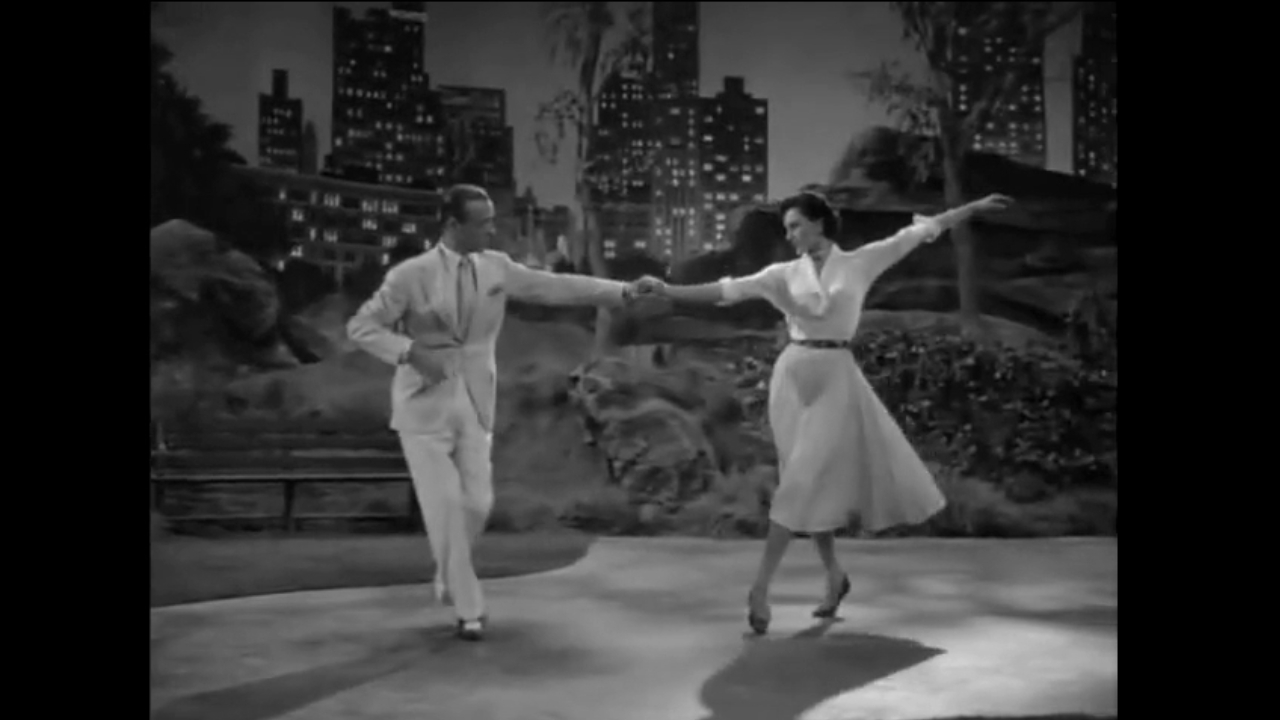
\includegraphics[scale=0.1]{img/bandwagon}
\caption{Dancing in the Dark.}
\end{wrapfigure}

There is a dance scene in the film ``The Band Wagon,'' where Cyd Charisse and Fred Astaire start out by walking together side by side, exchanging twirls until it morphs completely into a swing style dance. This scene is our use case for inventing a notation which extends seamlessly to more than one character.

To determine which poses for these dancers were common, I annotated the video with what I thought good keyframes would be if the two characters were treated as one. 

\begin{table}[!htb]
  \centering
  \begin{tabular}{ | c | c || c | c | c | }
    \hline
     & Separate & \multicolumn{3}{c |}{Together}\\ \hline
    1 LOA 
    & &
    \begin{minipage}{.15\textwidth}
      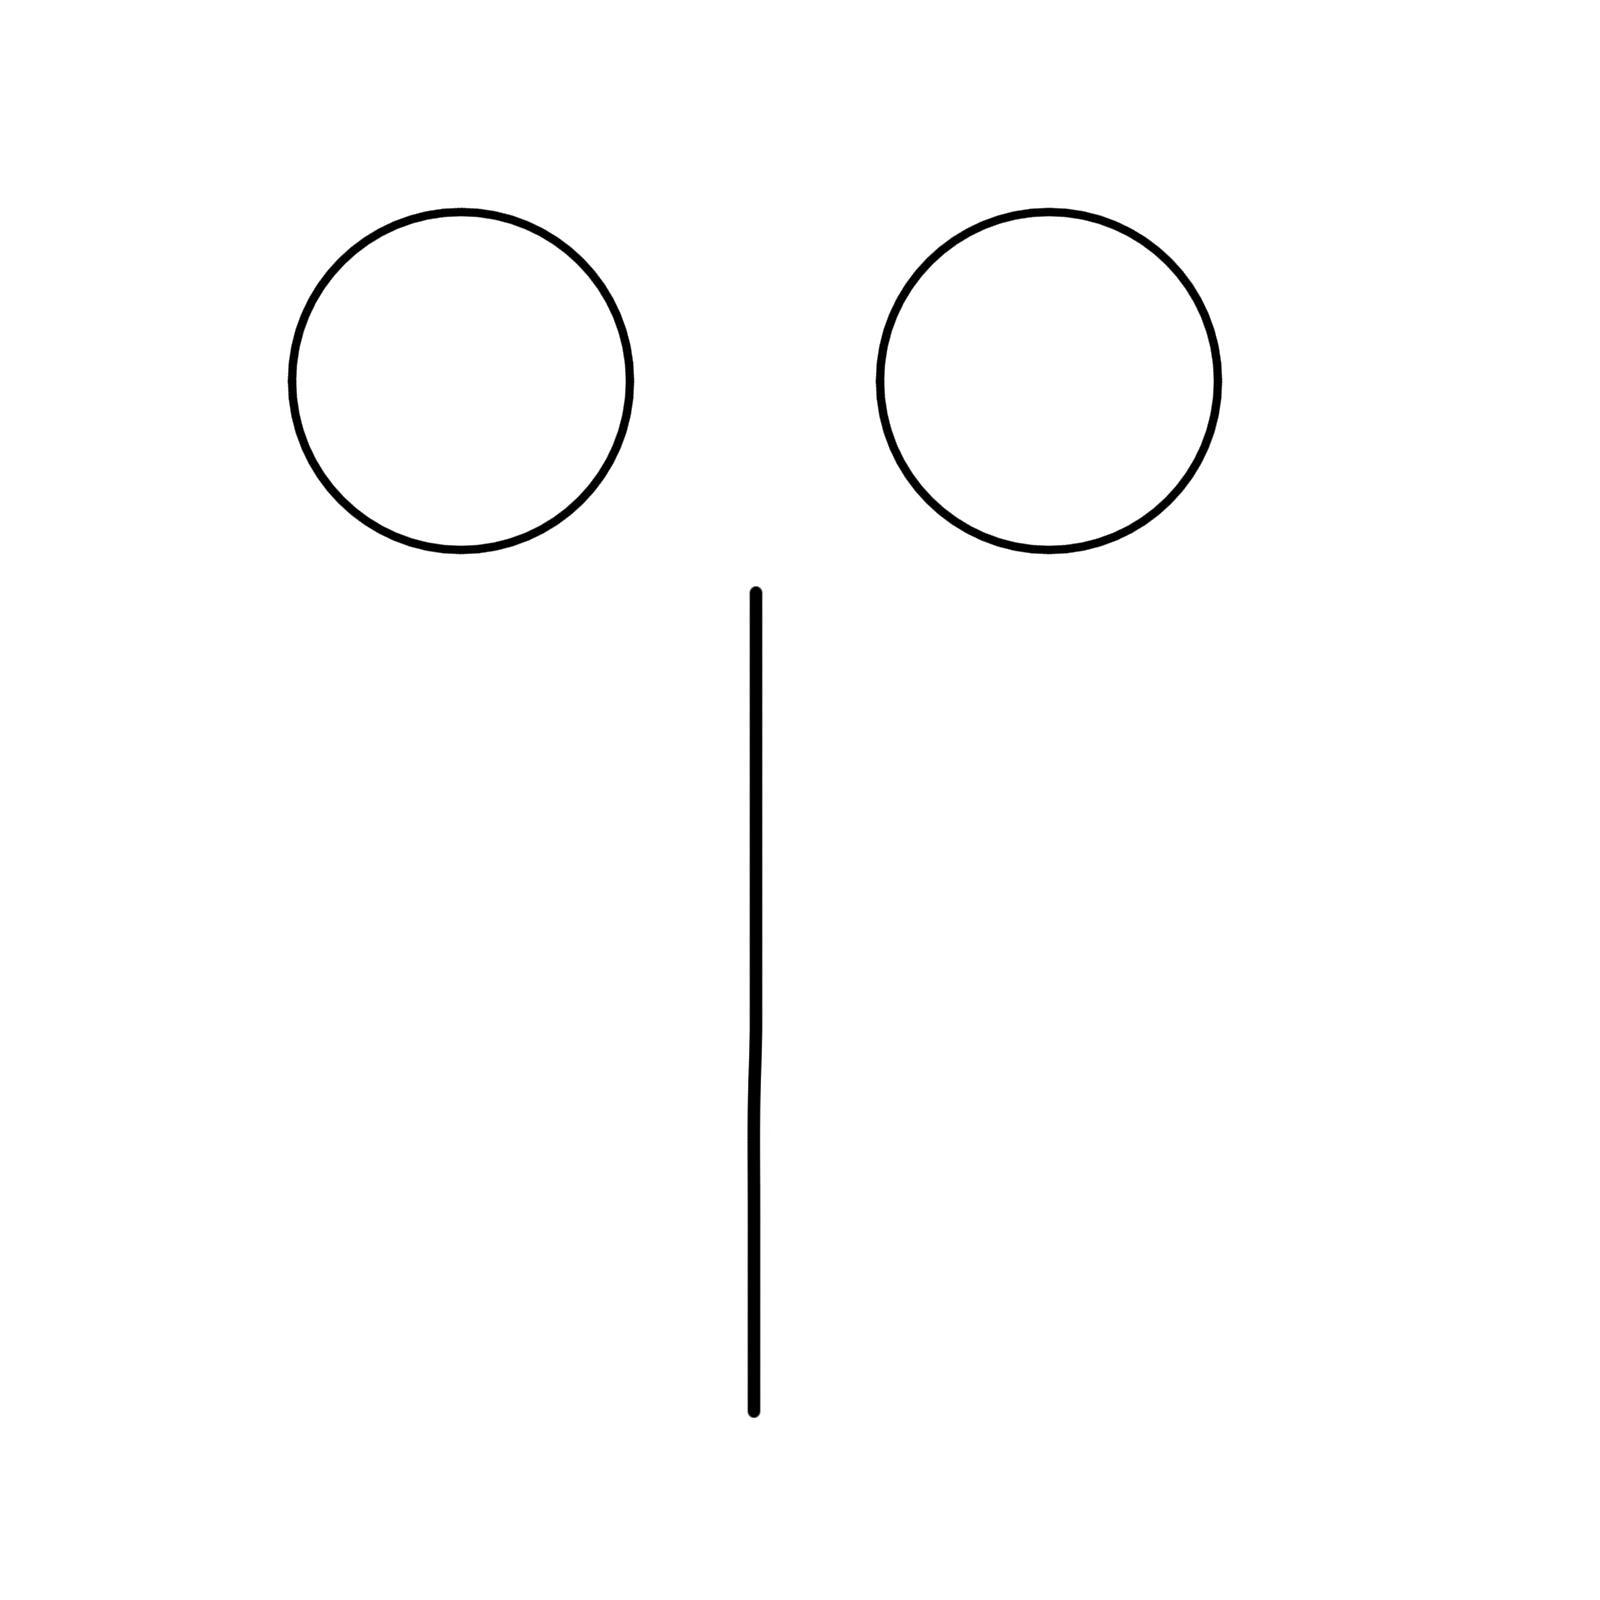
\includegraphics[width=\linewidth, height=20mm]{img/01keyframe}
    \end{minipage} & & \\ 
    \hline
    2 LOA 
    &
    \begin{minipage}{.15\textwidth}
      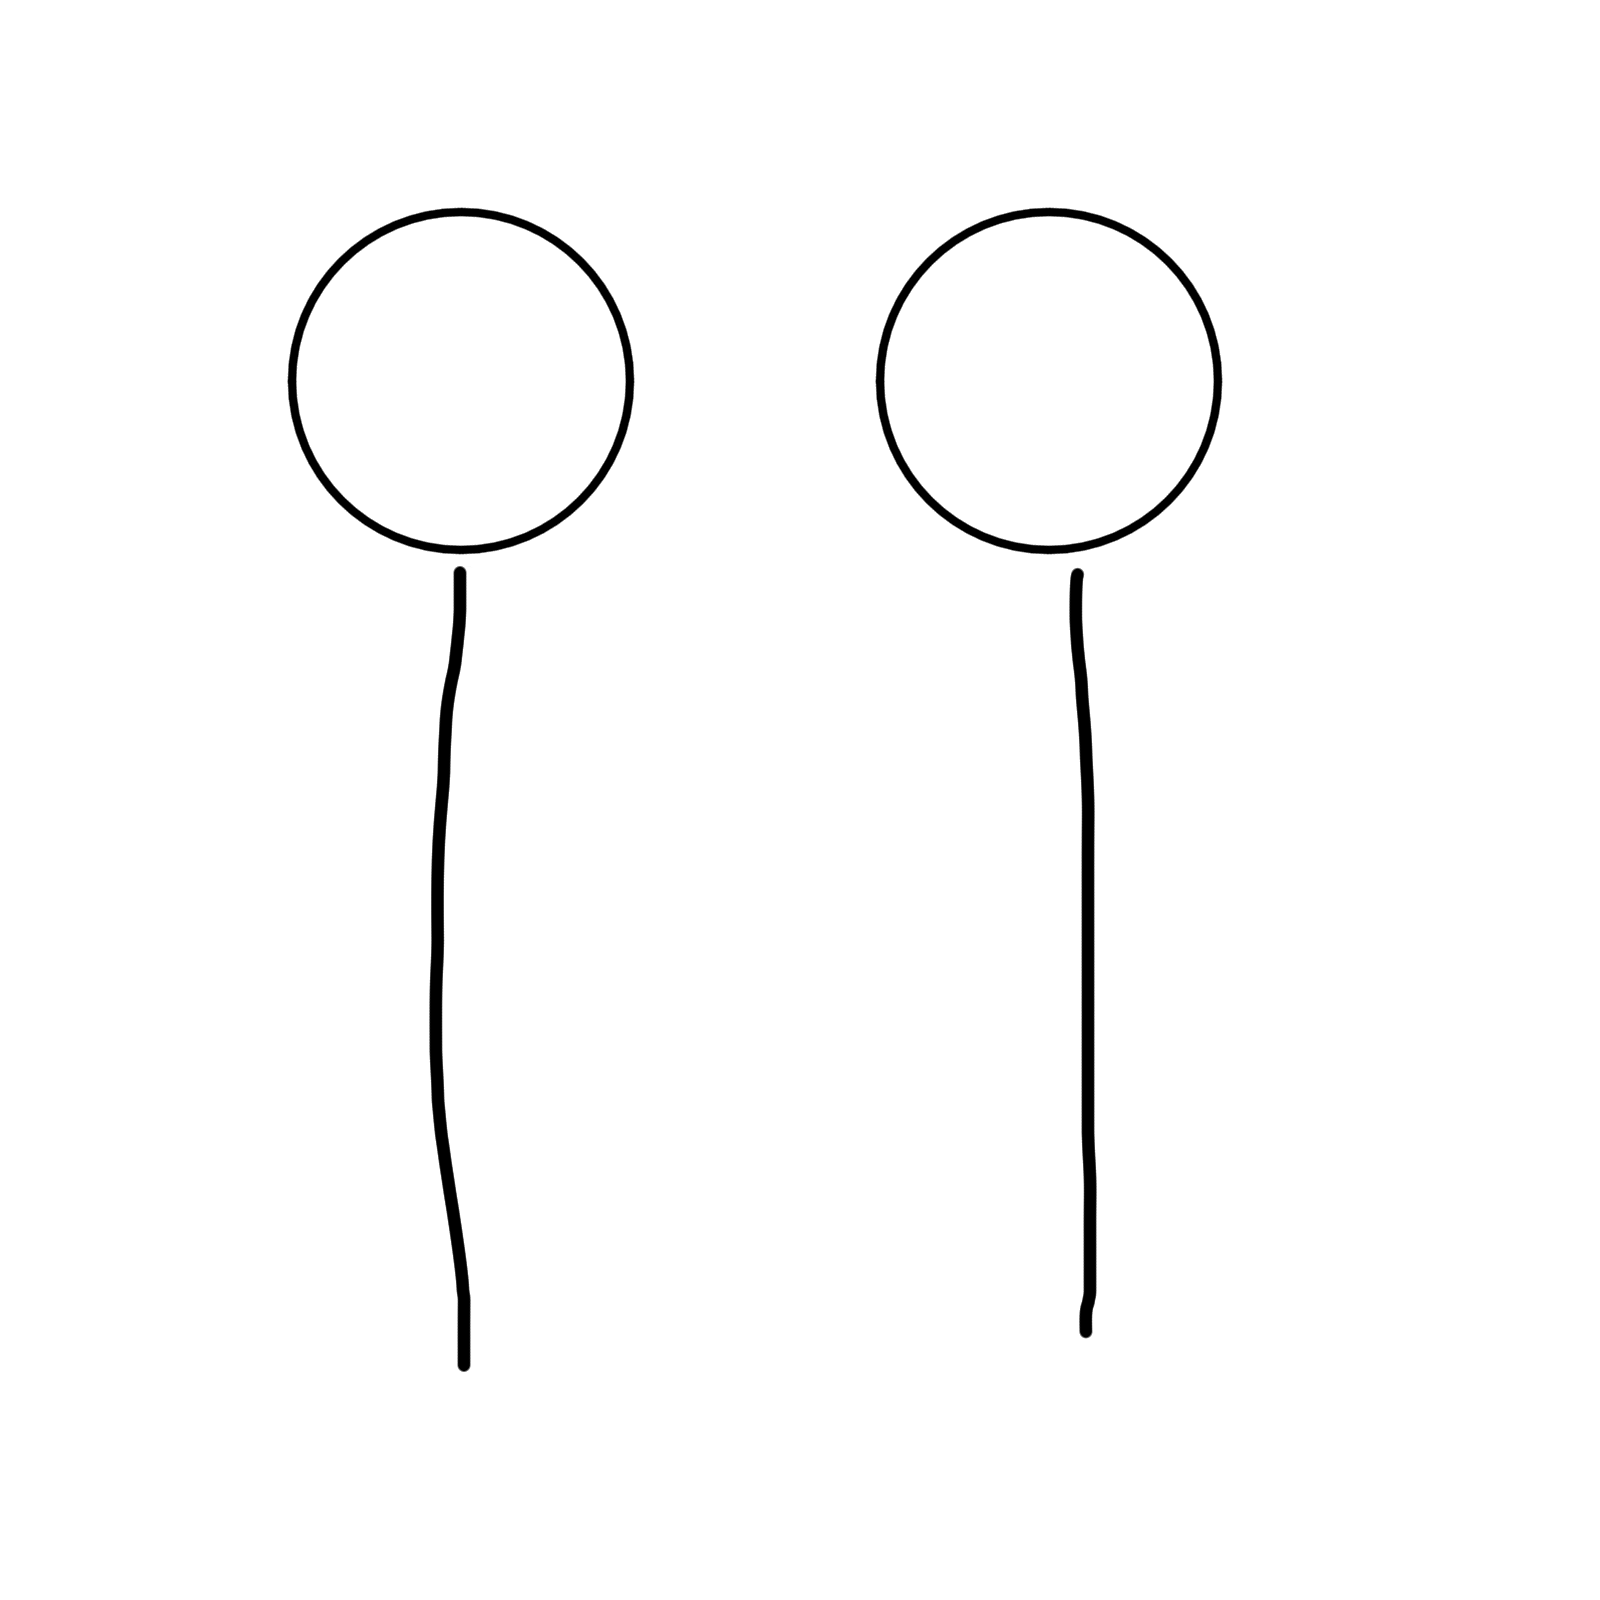
\includegraphics[width=\linewidth, height=20mm]{img/2loa_separate_keyframe}
    \end{minipage}
    &
    \begin{minipage}{.15\textwidth}
      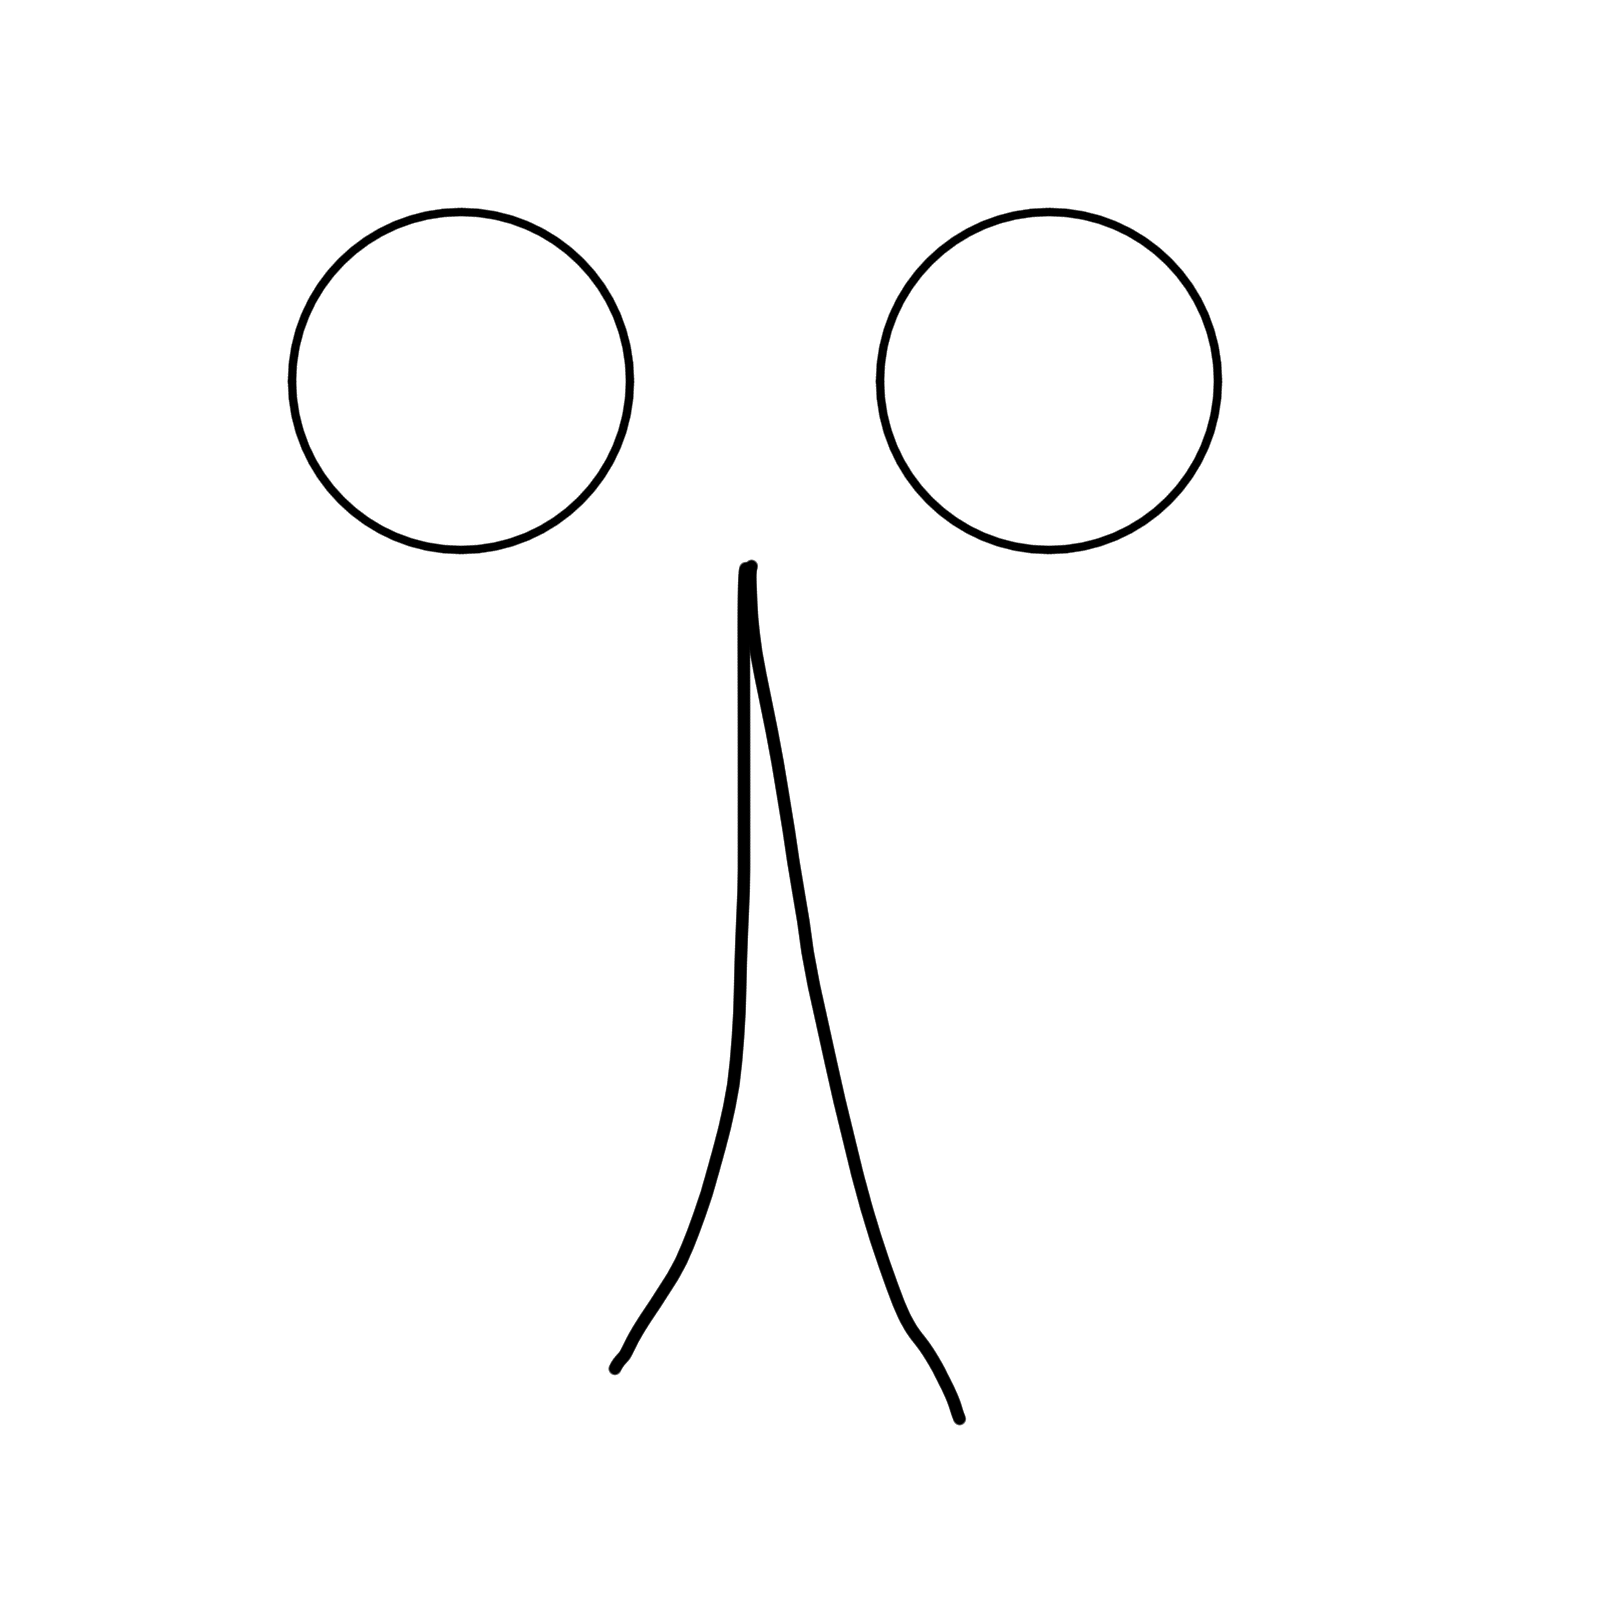
\includegraphics[width=\linewidth, height=20mm]{img/02keyframe}
    \end{minipage}
    &
    \begin{minipage}{.15\textwidth}
      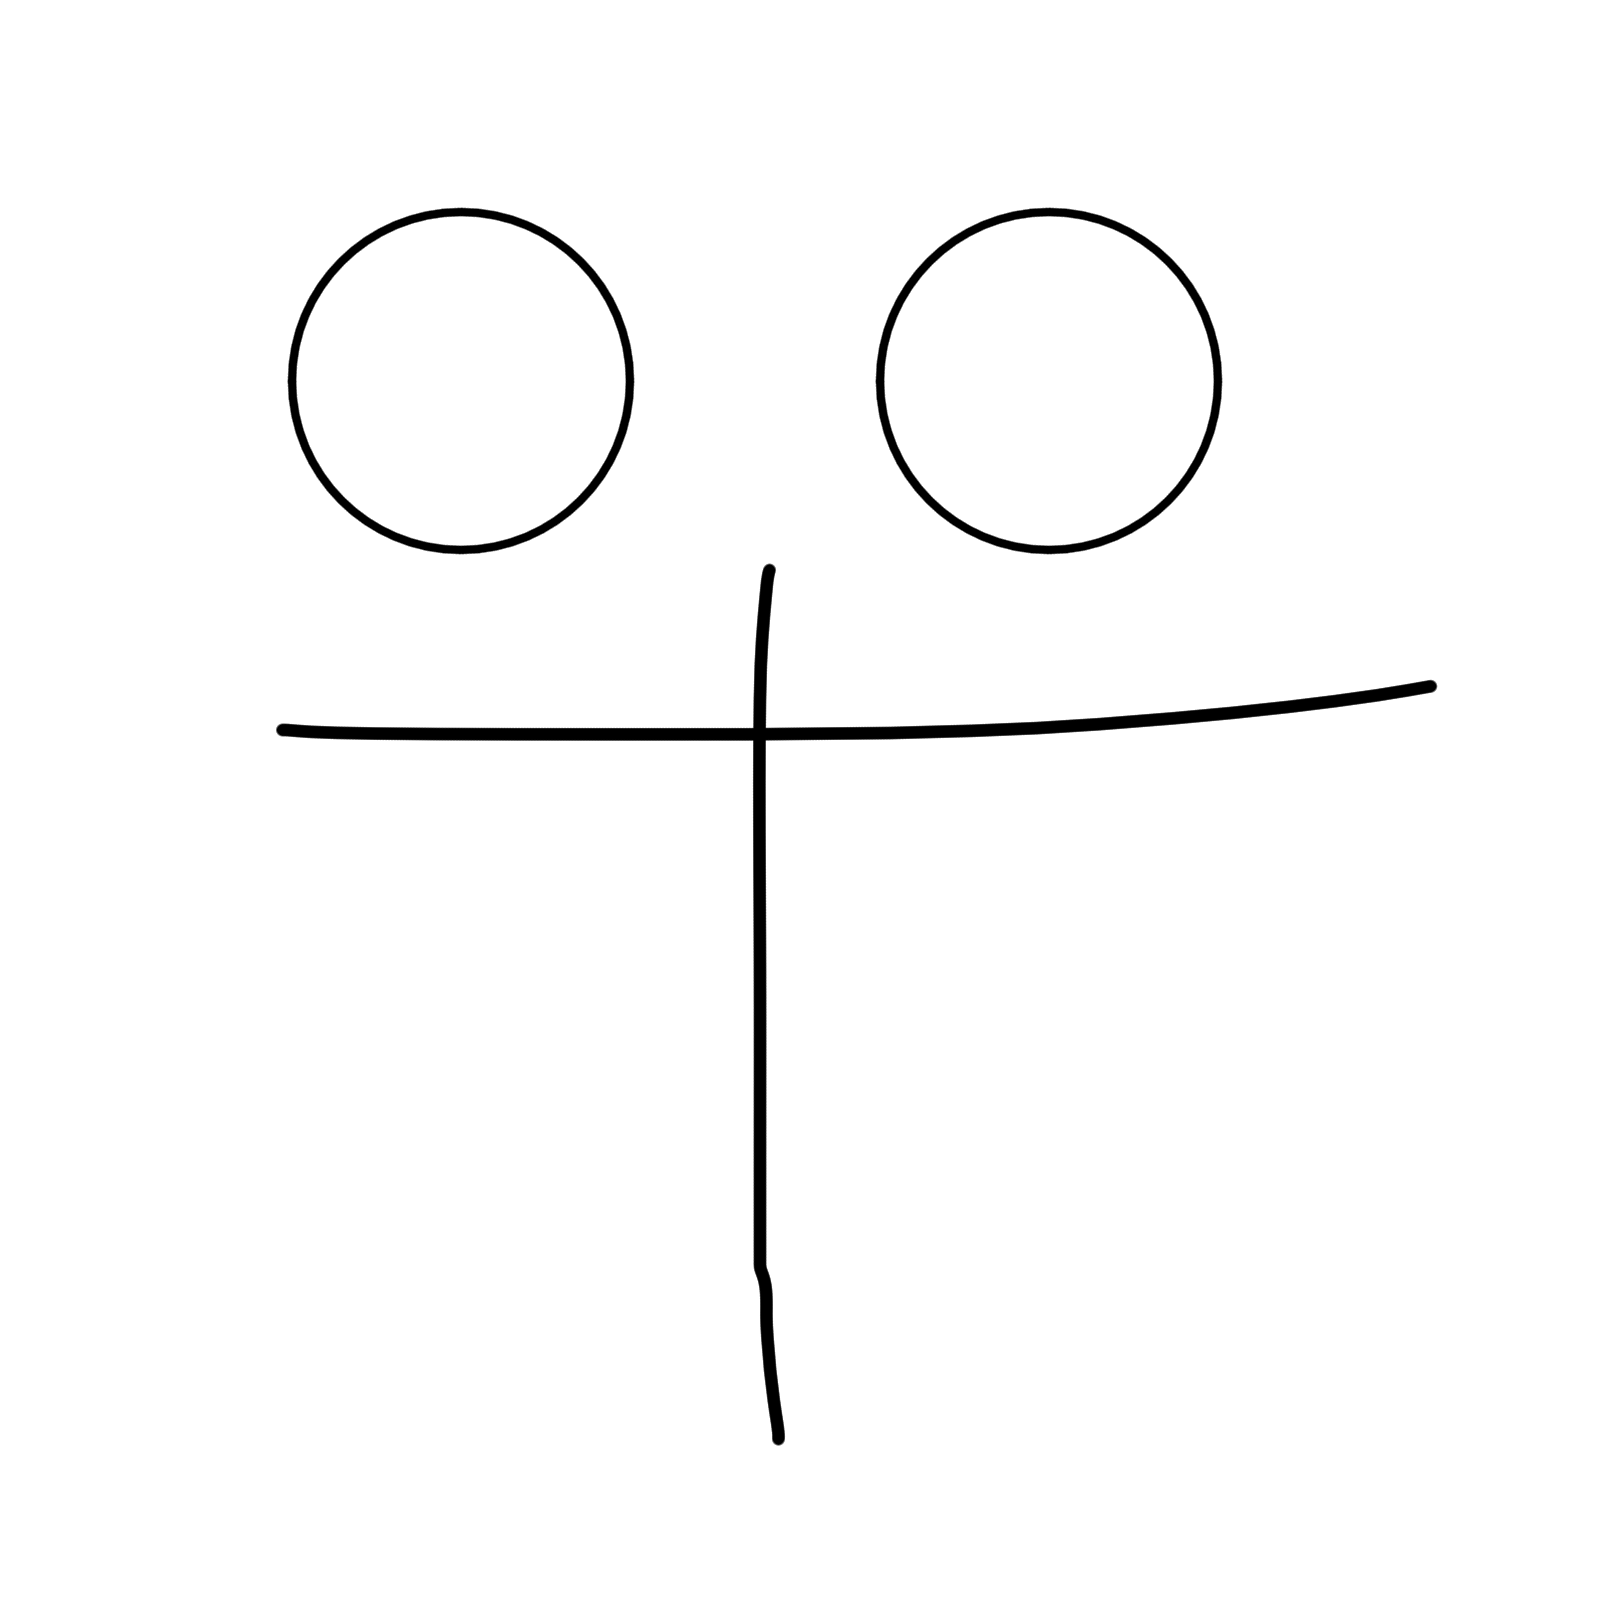
\includegraphics[width=\linewidth, height=20mm]{img/03keyframe}
    \end{minipage} & 
    \\ \hline
    3 LOA 
    &
    \begin{minipage}{.15\textwidth}
      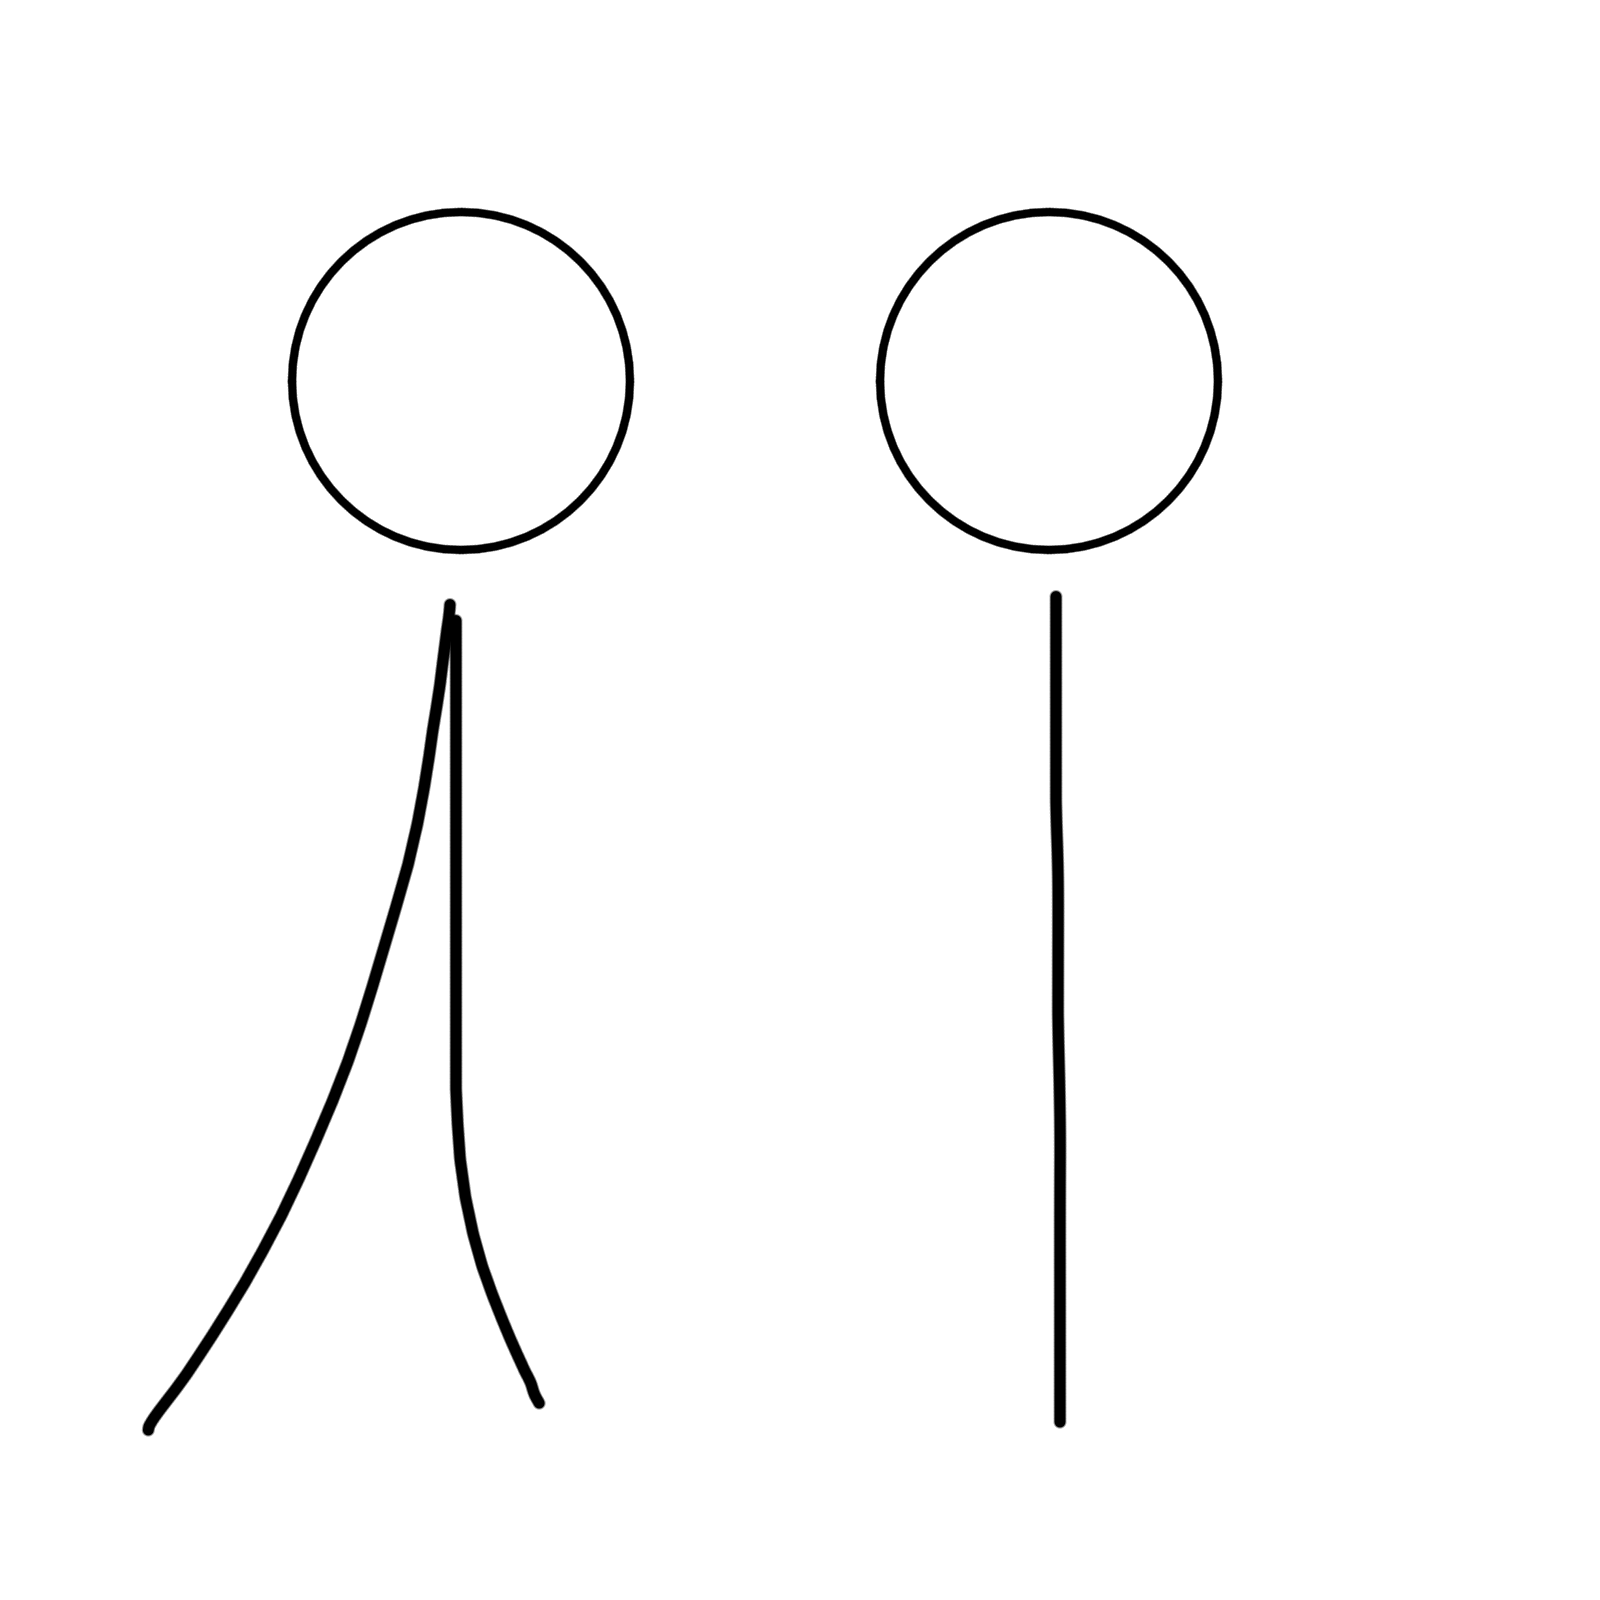
\includegraphics[width=\linewidth, height=20mm]{img/3loa_separate_keyframe}
    \end{minipage}
    &
    \begin{minipage}{.15\textwidth}
      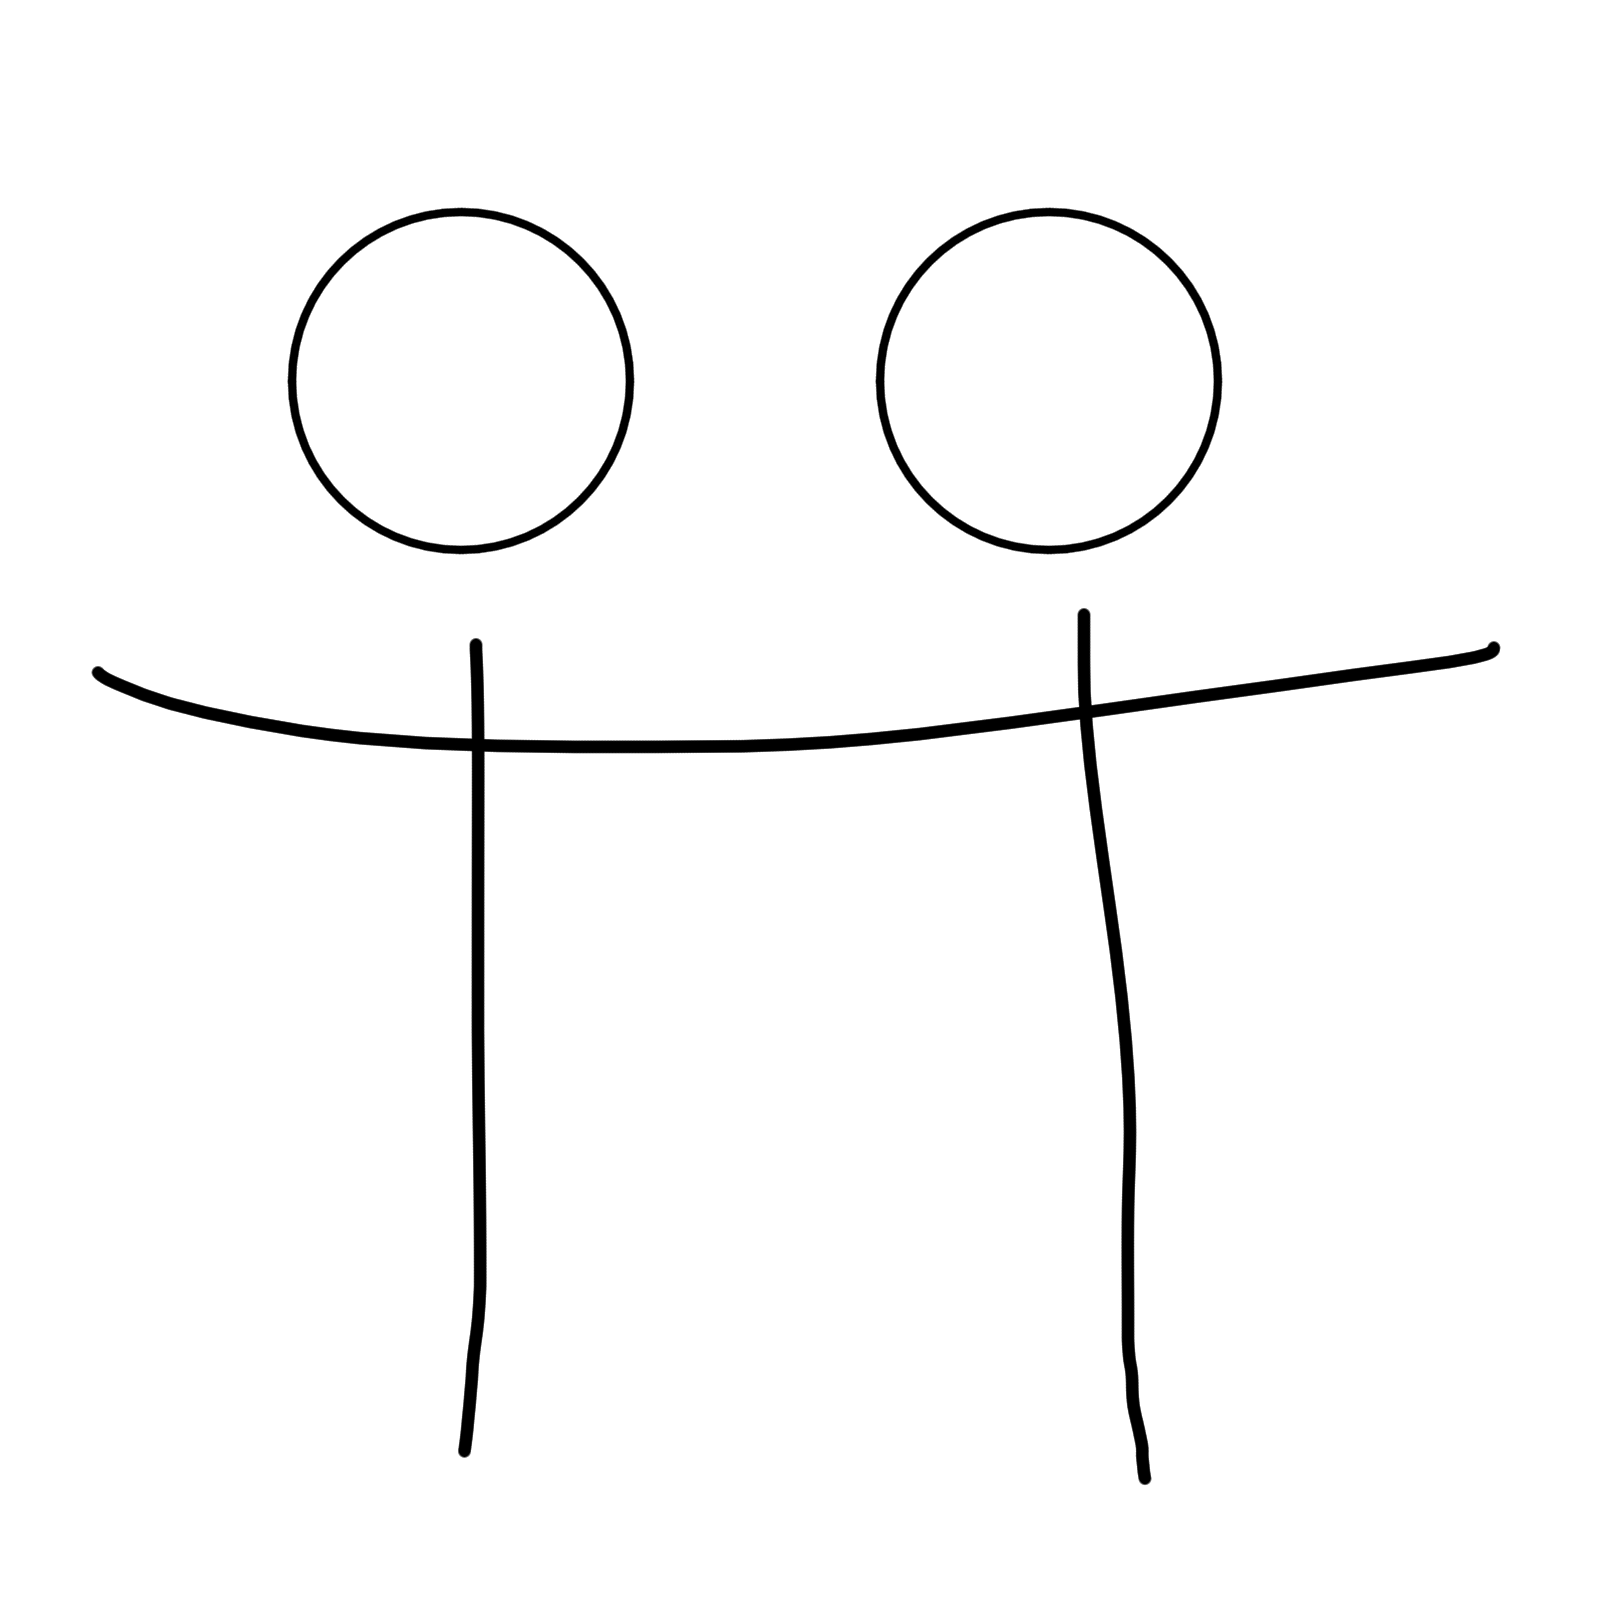
\includegraphics[width=\linewidth, height=20mm]{img/04keyframe}
    \end{minipage}
    &
    \begin{minipage}{.15\textwidth}
      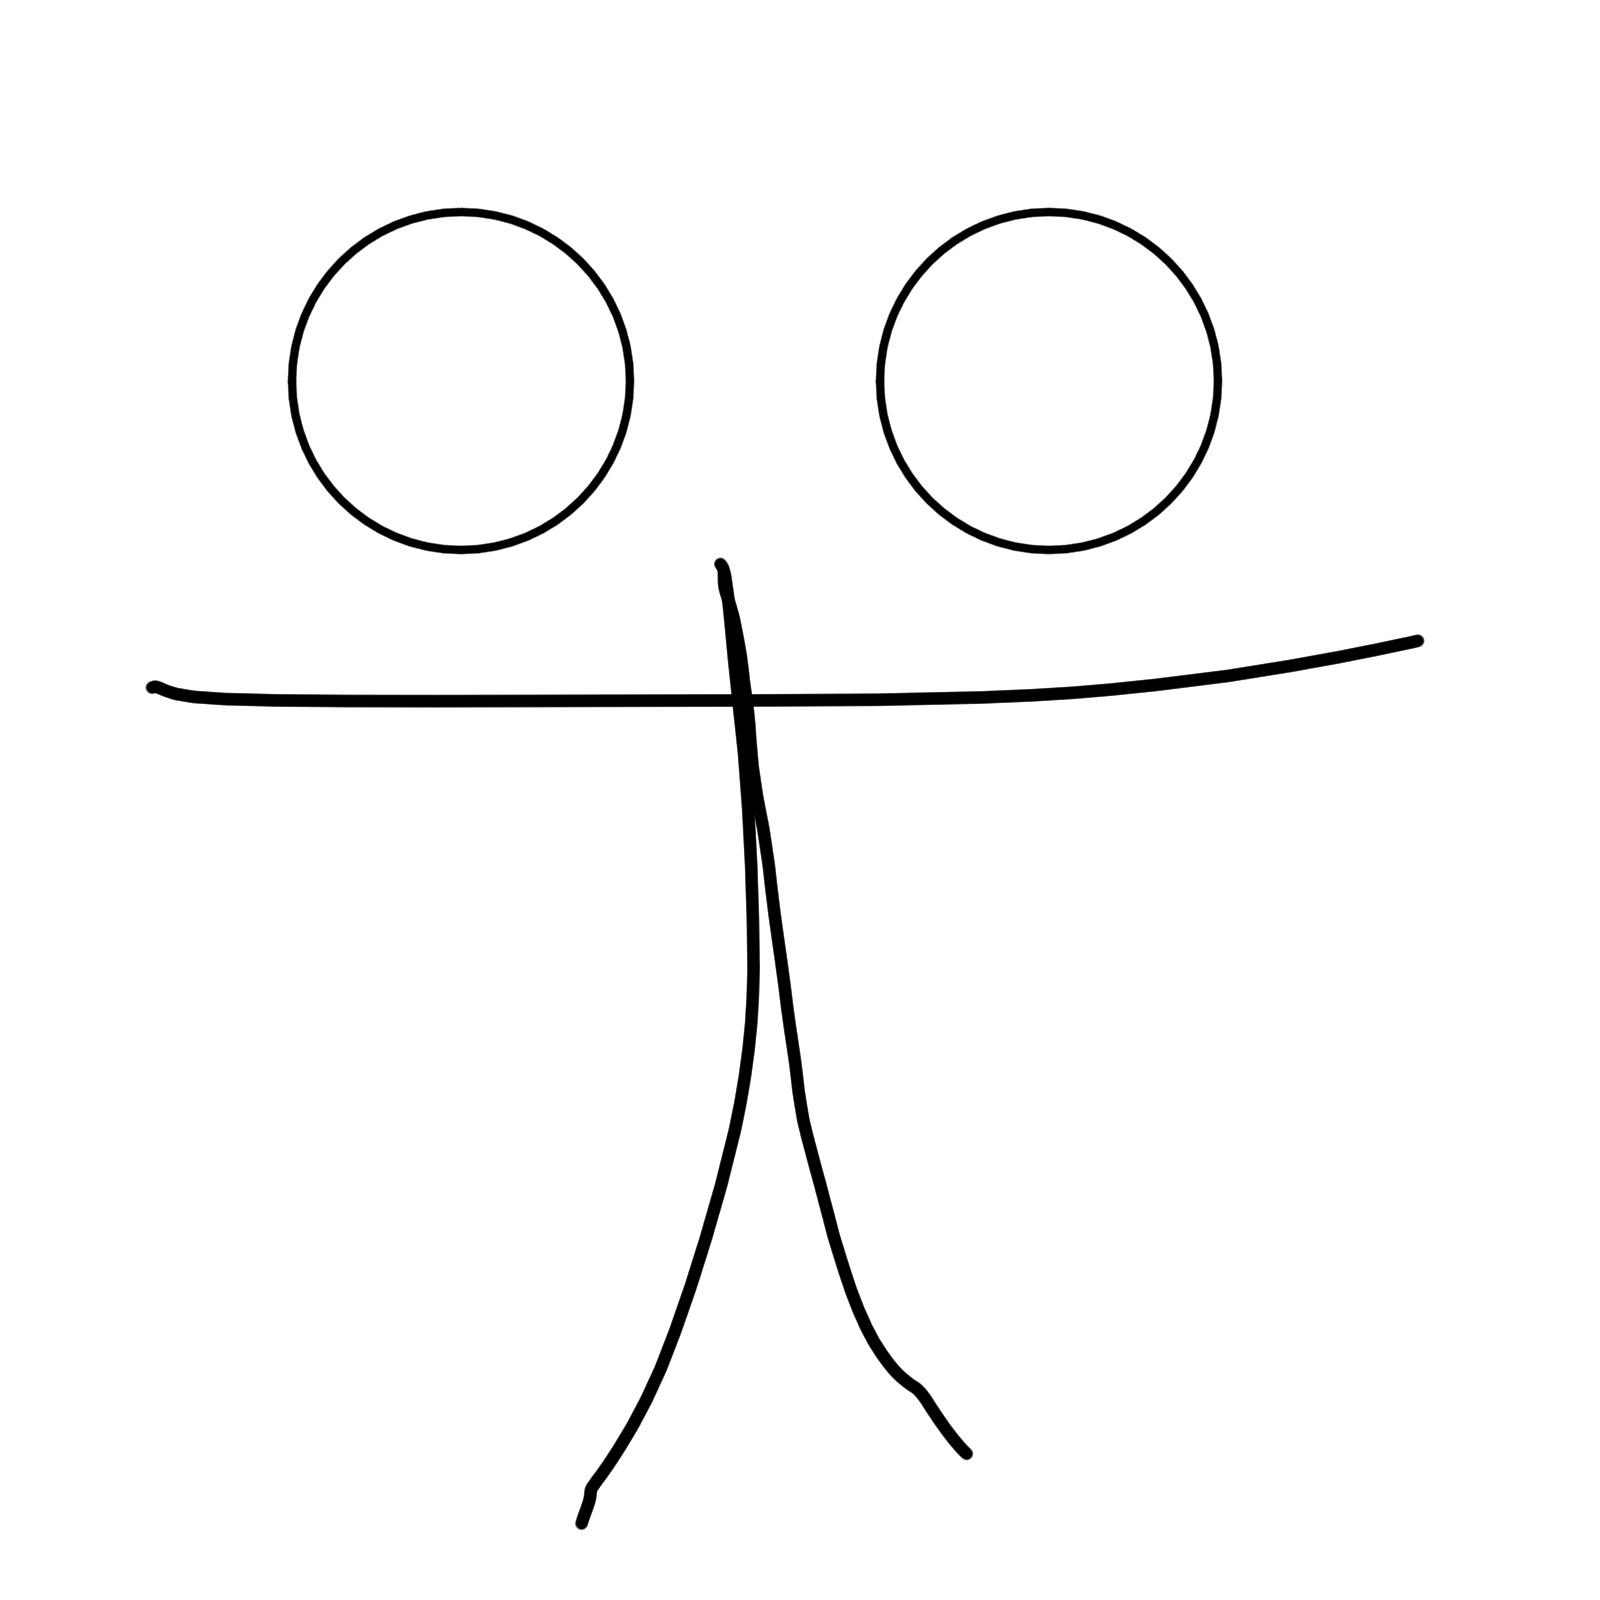
\includegraphics[width=\linewidth, height=20mm]{img/05keyframe}
    \end{minipage} 
    & 
    \begin{minipage}{.15\textwidth}
      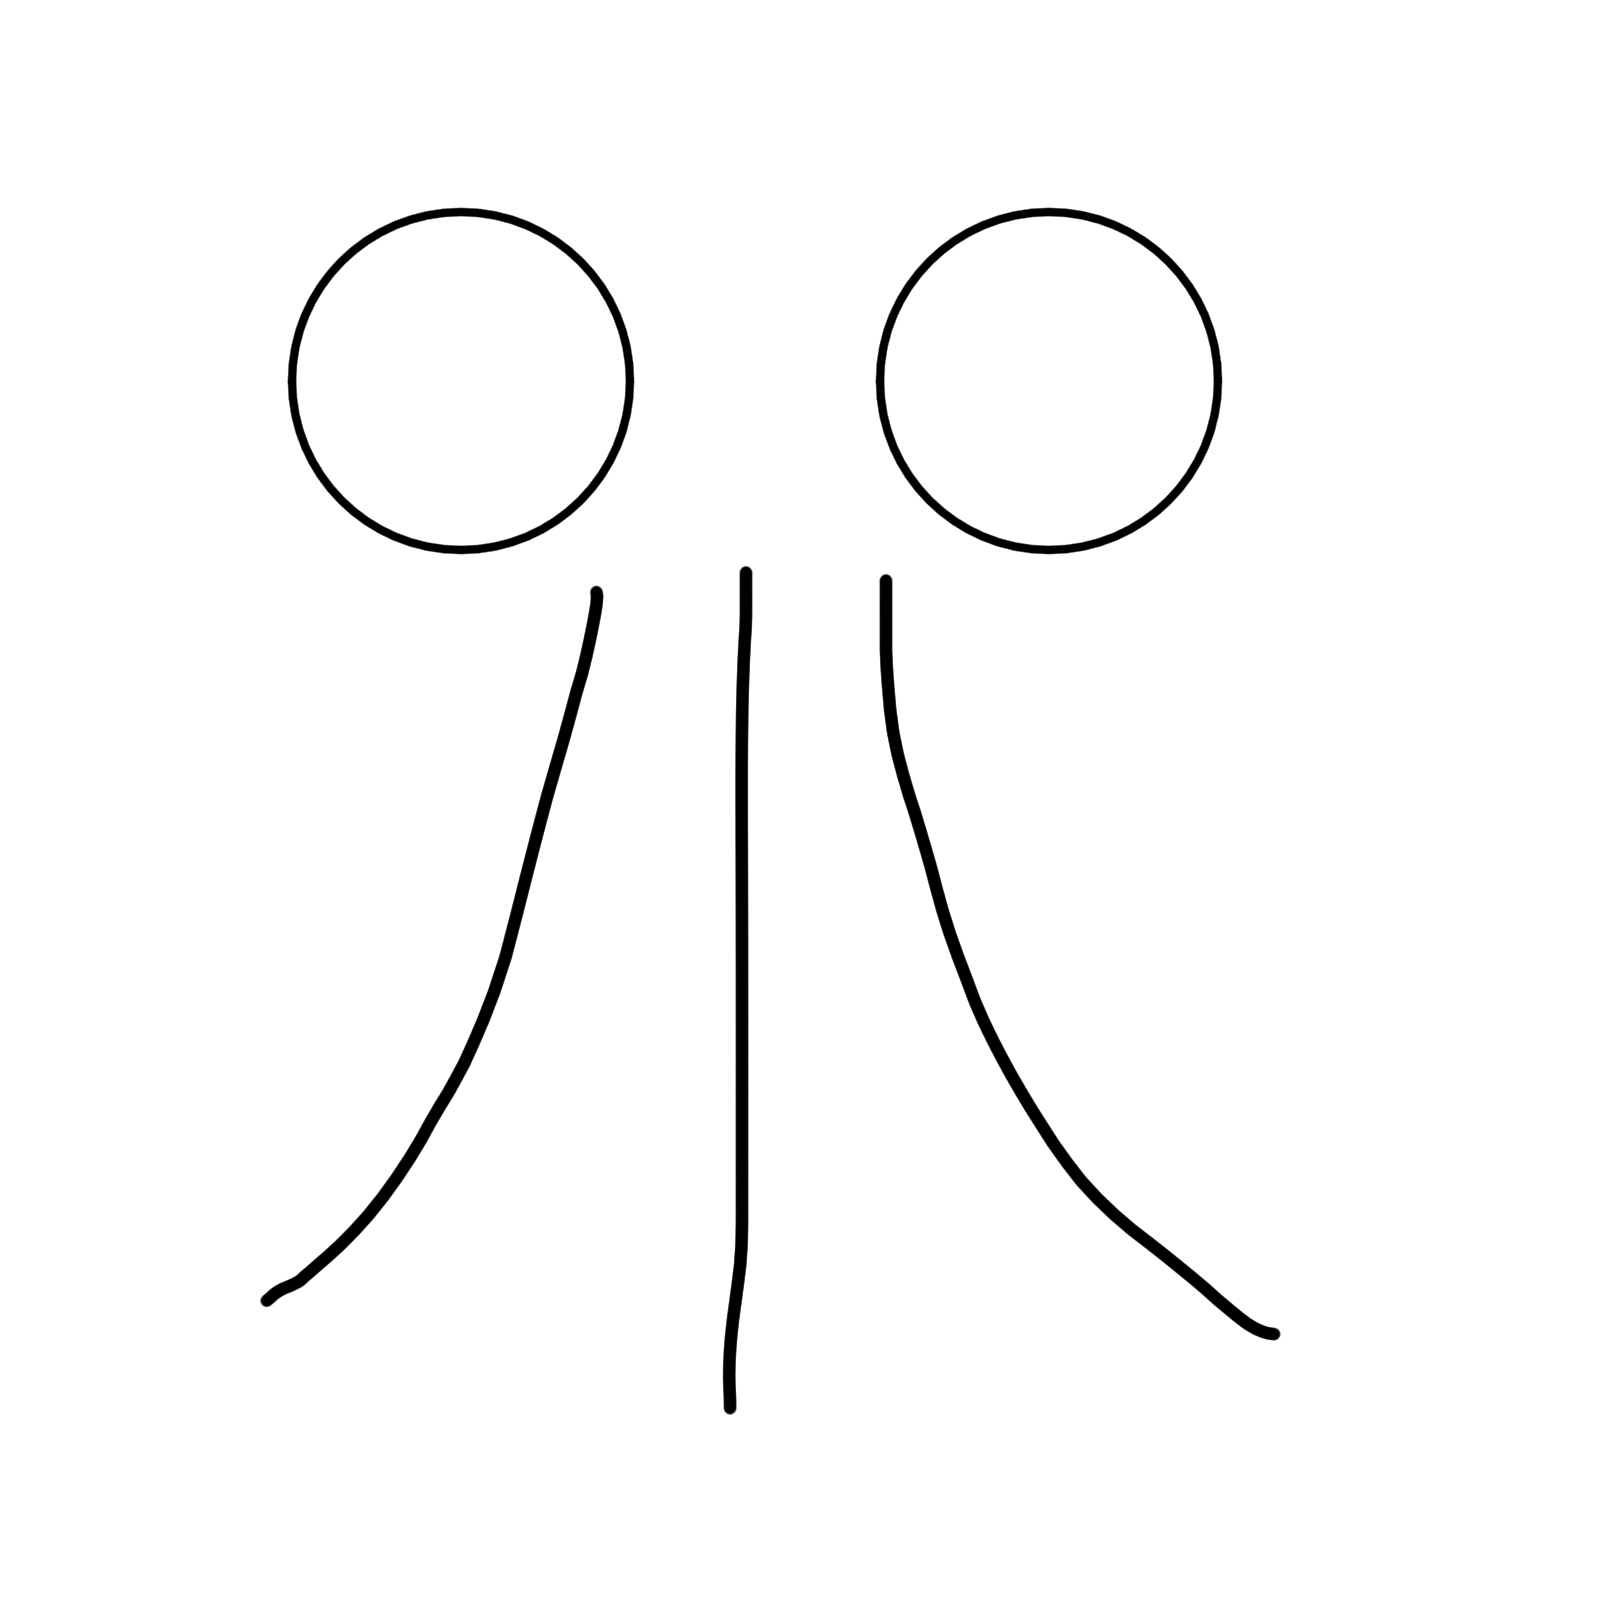
\includegraphics[width=\linewidth, height=20mm]{img/06keyframe}
    \end{minipage} 
    \\ \hline
    4 LOA 
    &
    \begin{minipage}{.15\textwidth}
      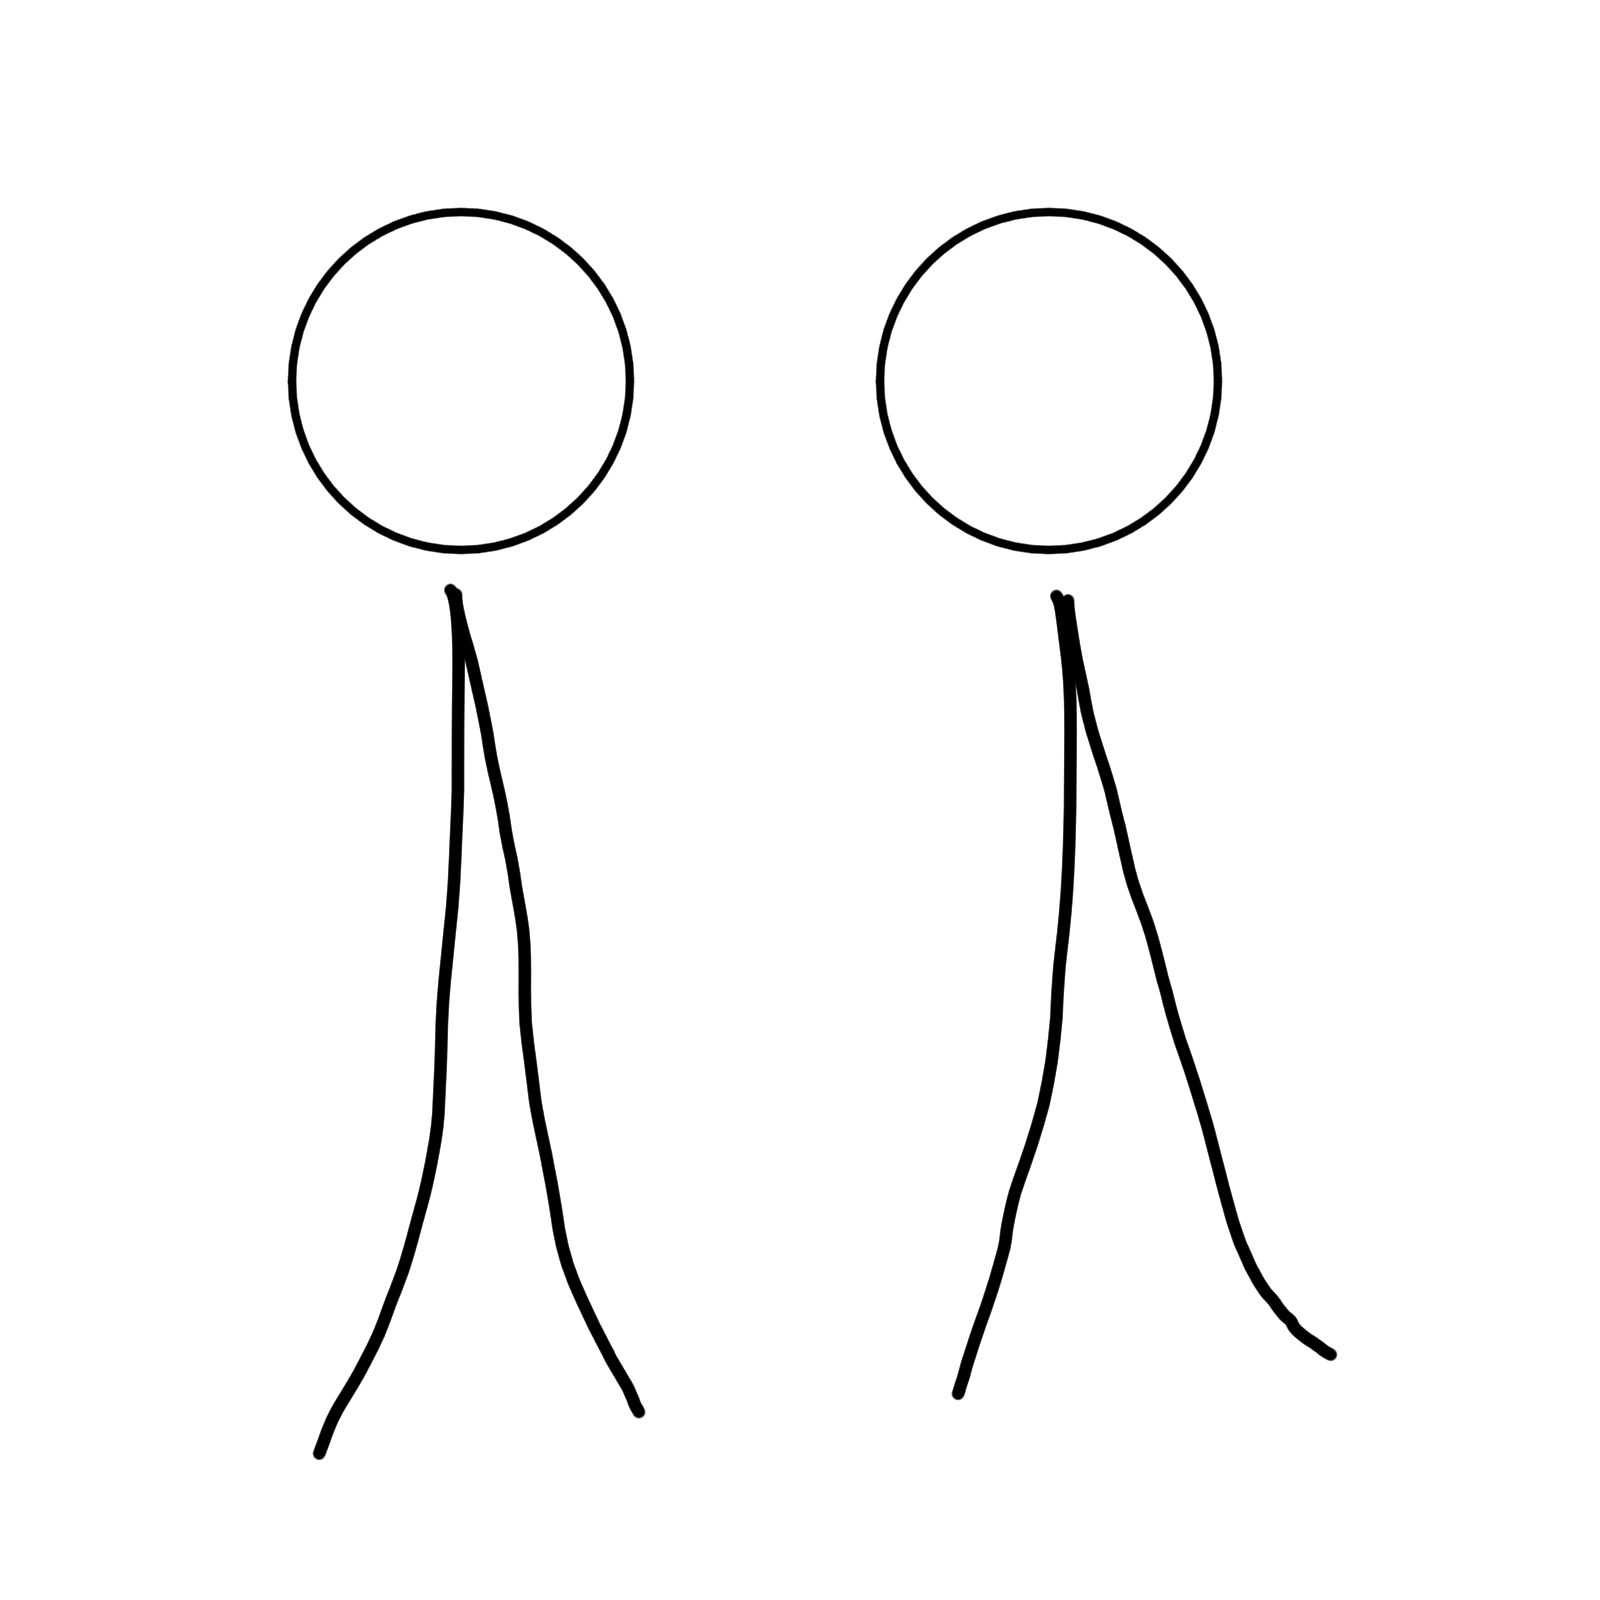
\includegraphics[width=\linewidth, height=20mm]{img/4loa_separate_keyframe}
    \end{minipage}
    &
    \begin{minipage}{.15\textwidth}
      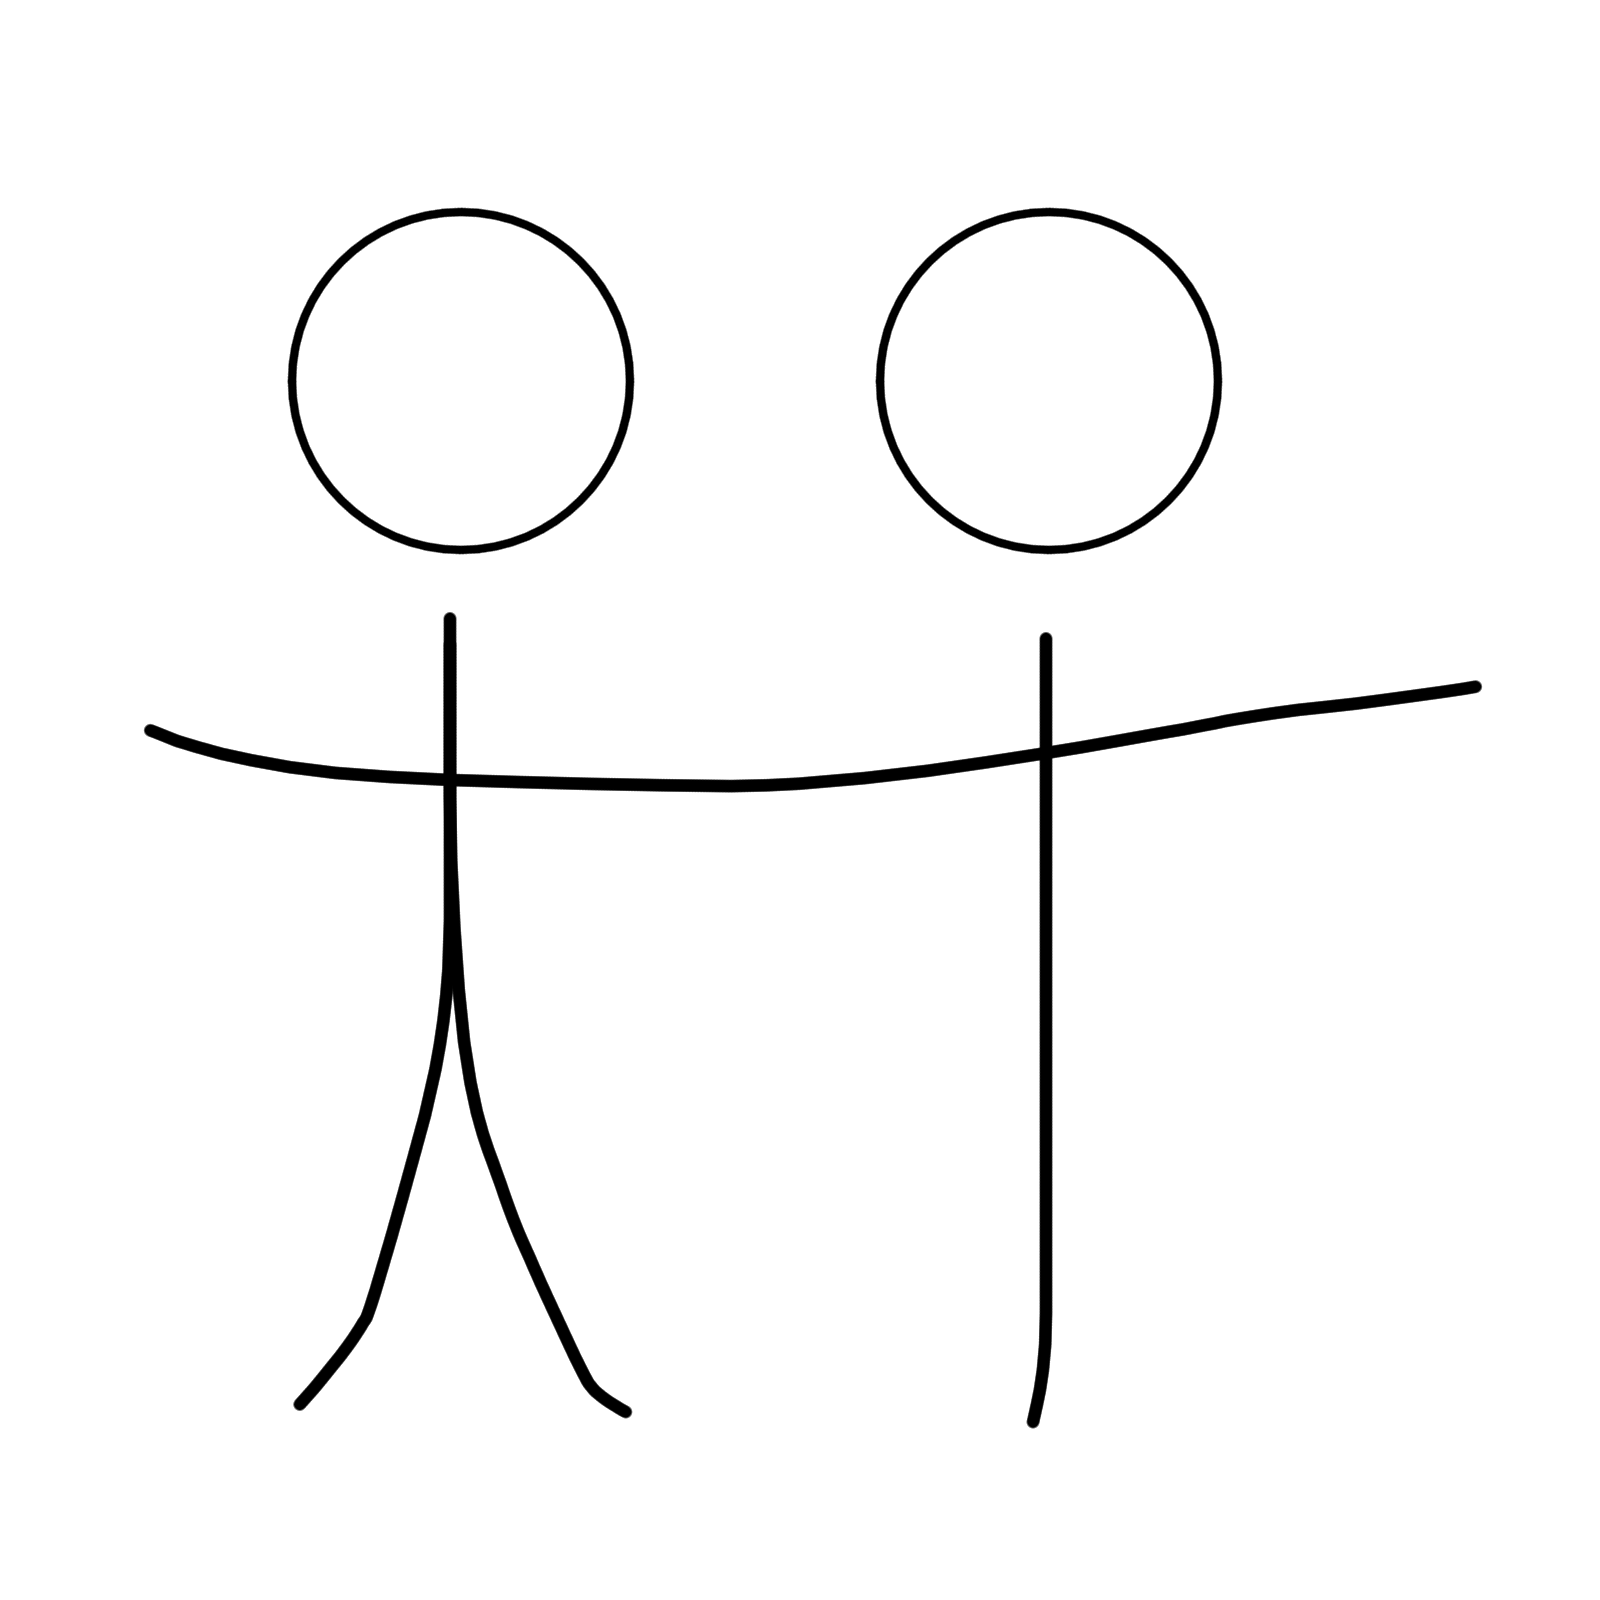
\includegraphics[width=\linewidth, height=20mm]{img/07keyframe}
    \end{minipage}
    &
    \begin{minipage}{.15\textwidth}
      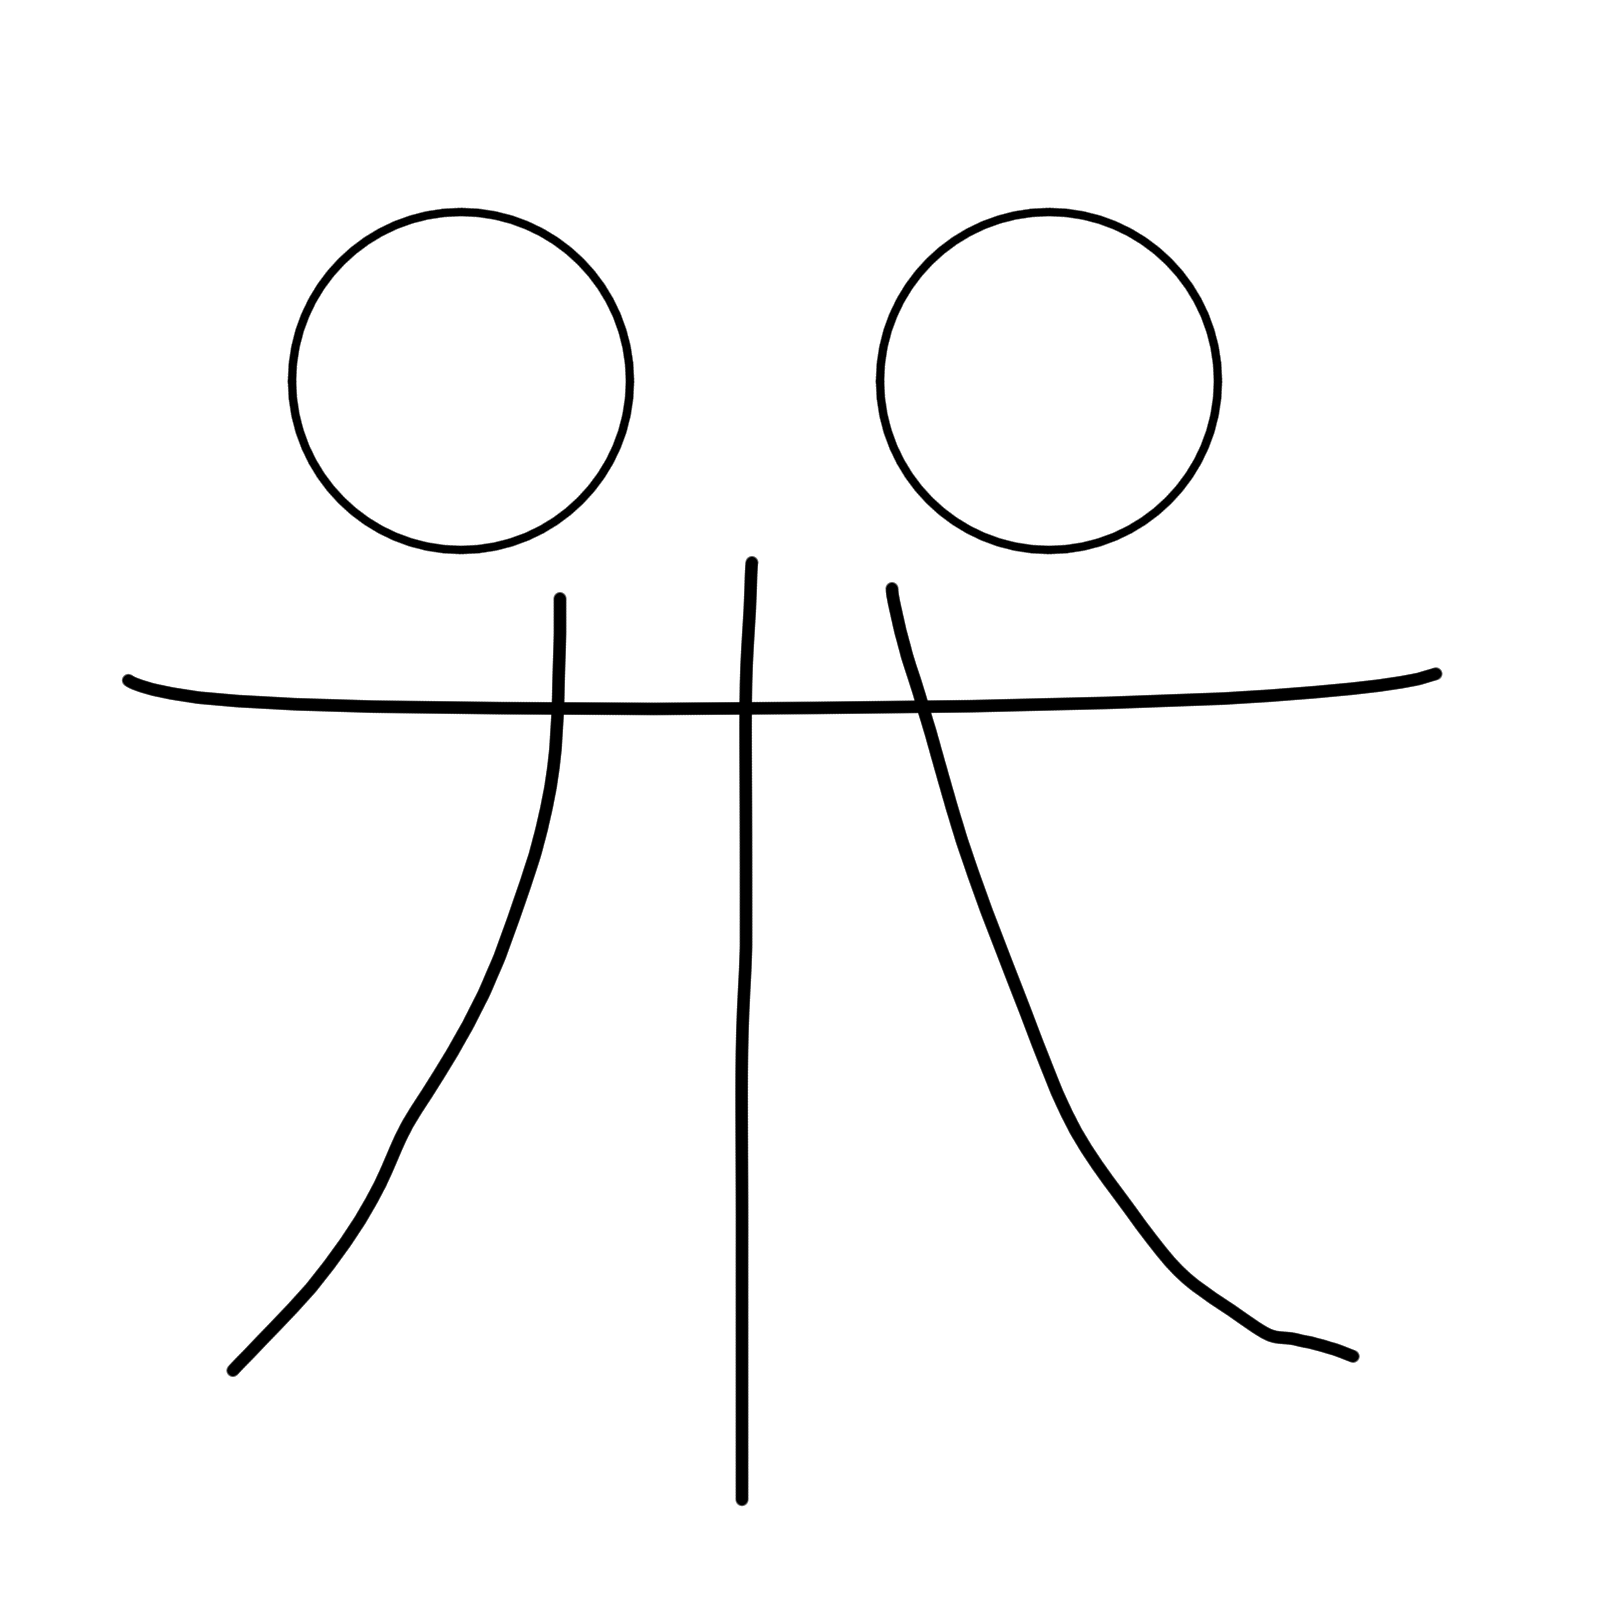
\includegraphics[width=\linewidth, height=20mm]{img/08keyframe}
    \end{minipage} 
    & 
    \begin{minipage}{.15\textwidth}
      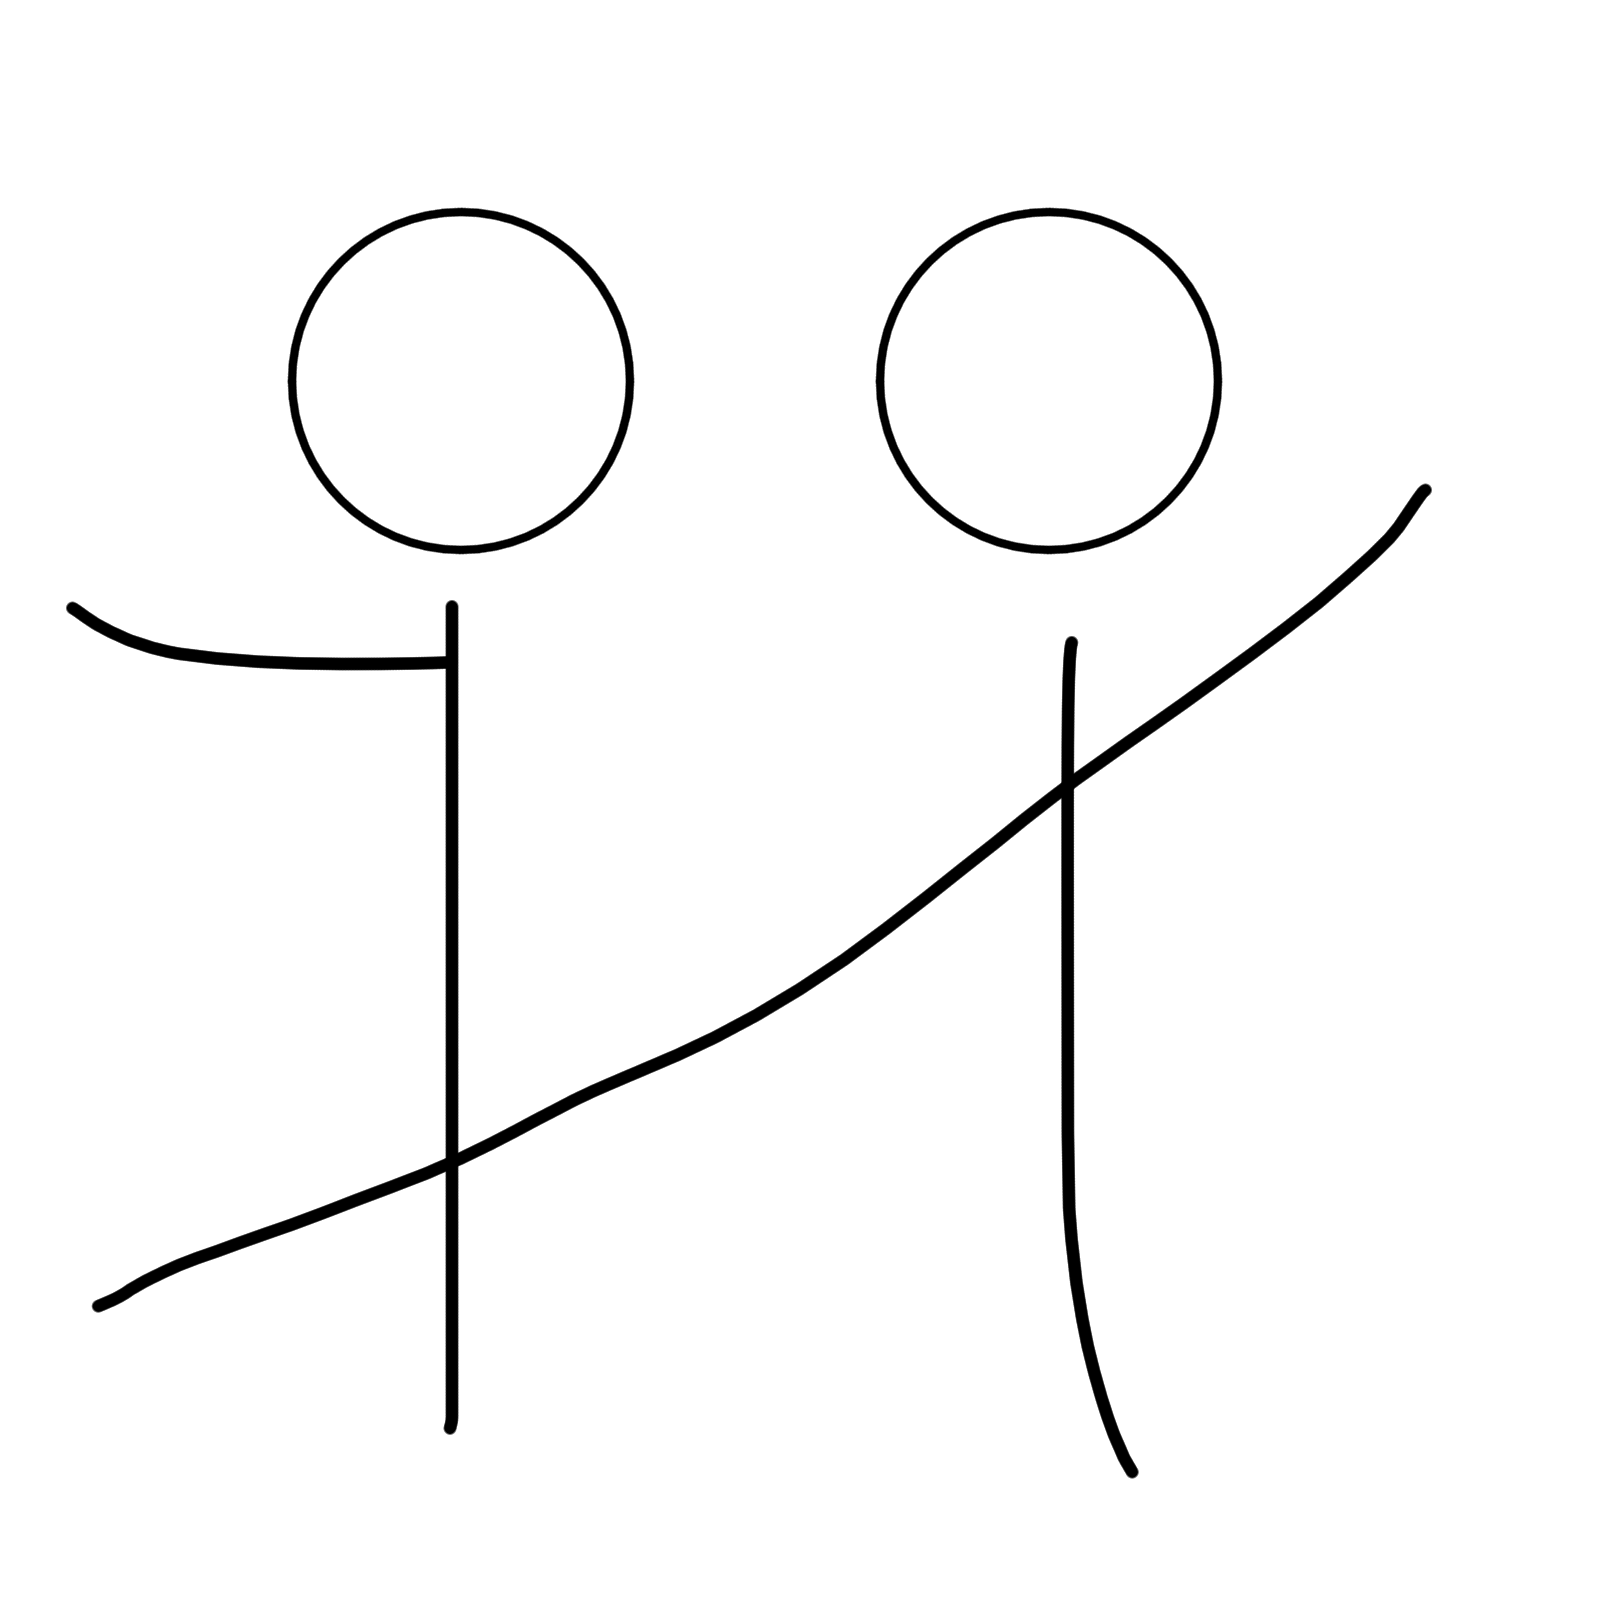
\includegraphics[width=\linewidth, height=20mm]{img/09keyframe}
    \end{minipage} 
    \\ \hline 
    &
    \begin{minipage}{.15\textwidth}
      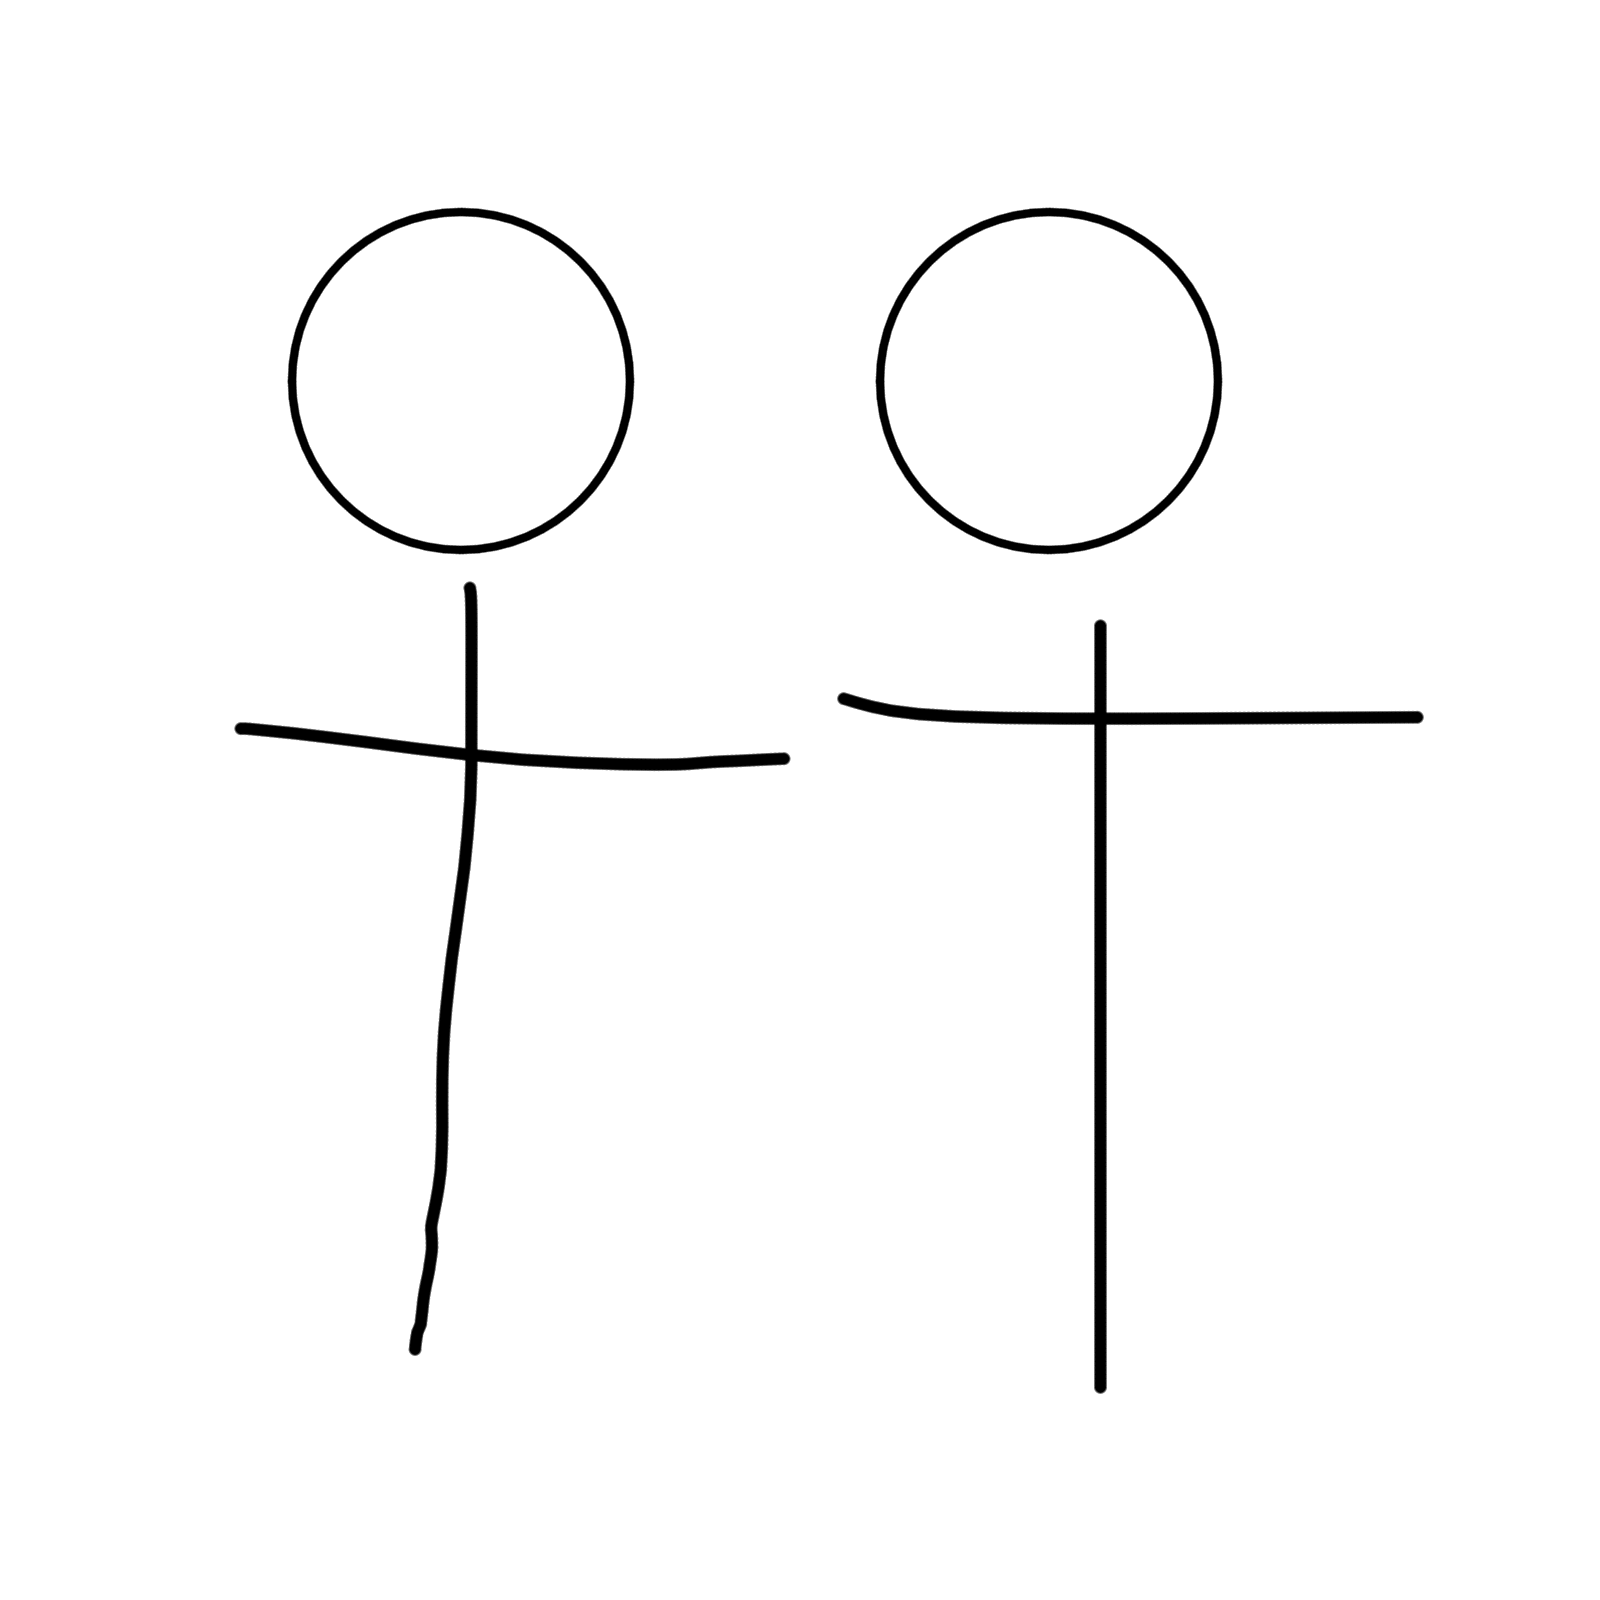
\includegraphics[width=\linewidth, height=20mm]{img/4-1loa_separate_keyframe}
    \end{minipage}
    & & & 
    \\ \hline
    5 LOA 
    &
    \begin{minipage}{.15\textwidth}
      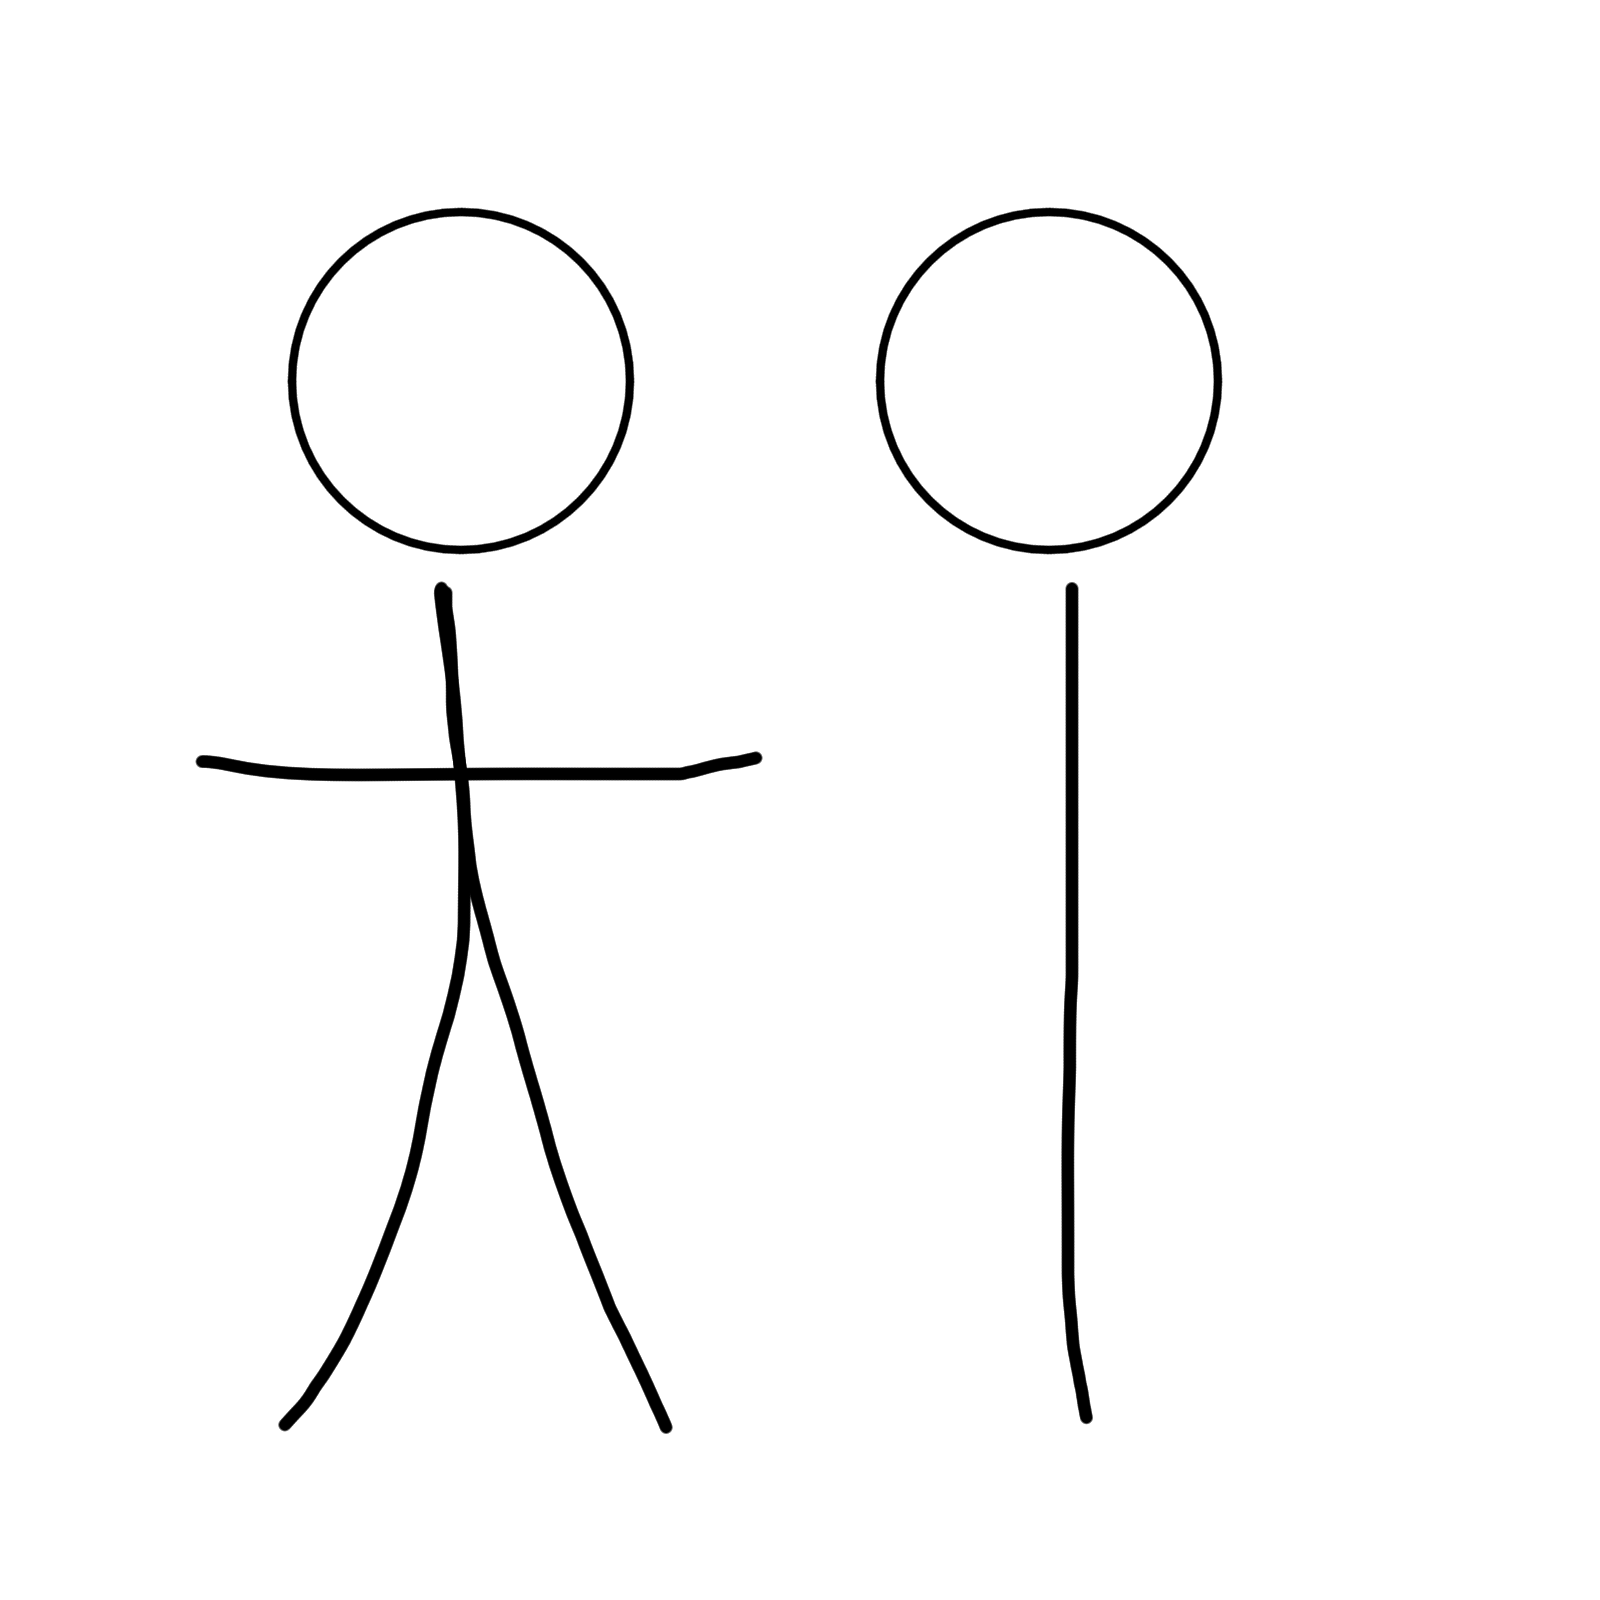
\includegraphics[width=\linewidth, height=20mm]{img/5loa_separate_keyframe}
    \end{minipage}
    &
    \begin{minipage}{.15\textwidth}
      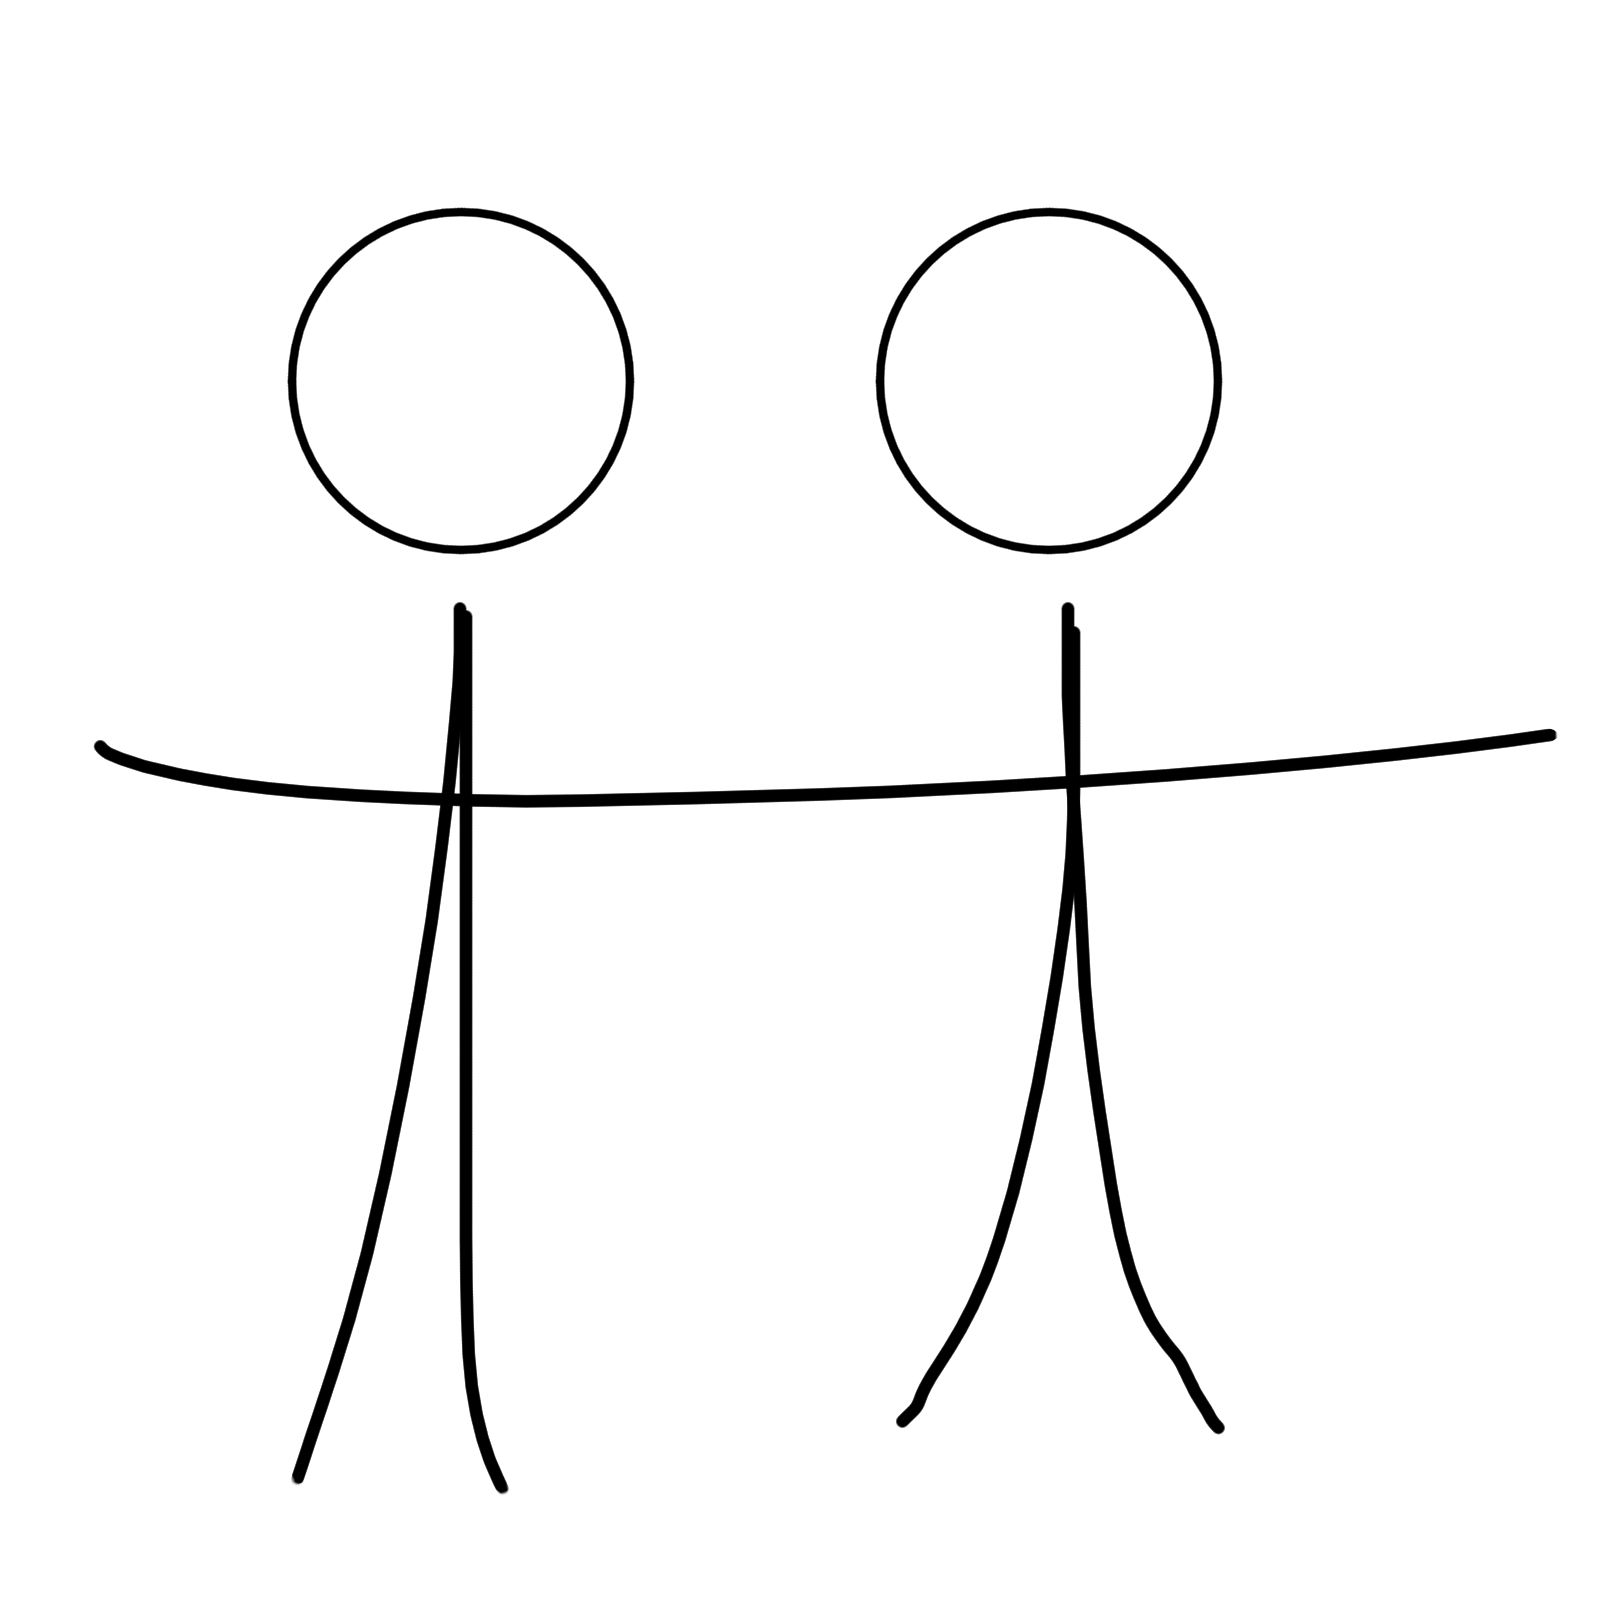
\includegraphics[width=\linewidth, height=20mm]{img/10keyframe}
    \end{minipage} & & 
    \\ \hline
    6 LOA 
    &
    \begin{minipage}{.15\textwidth}
      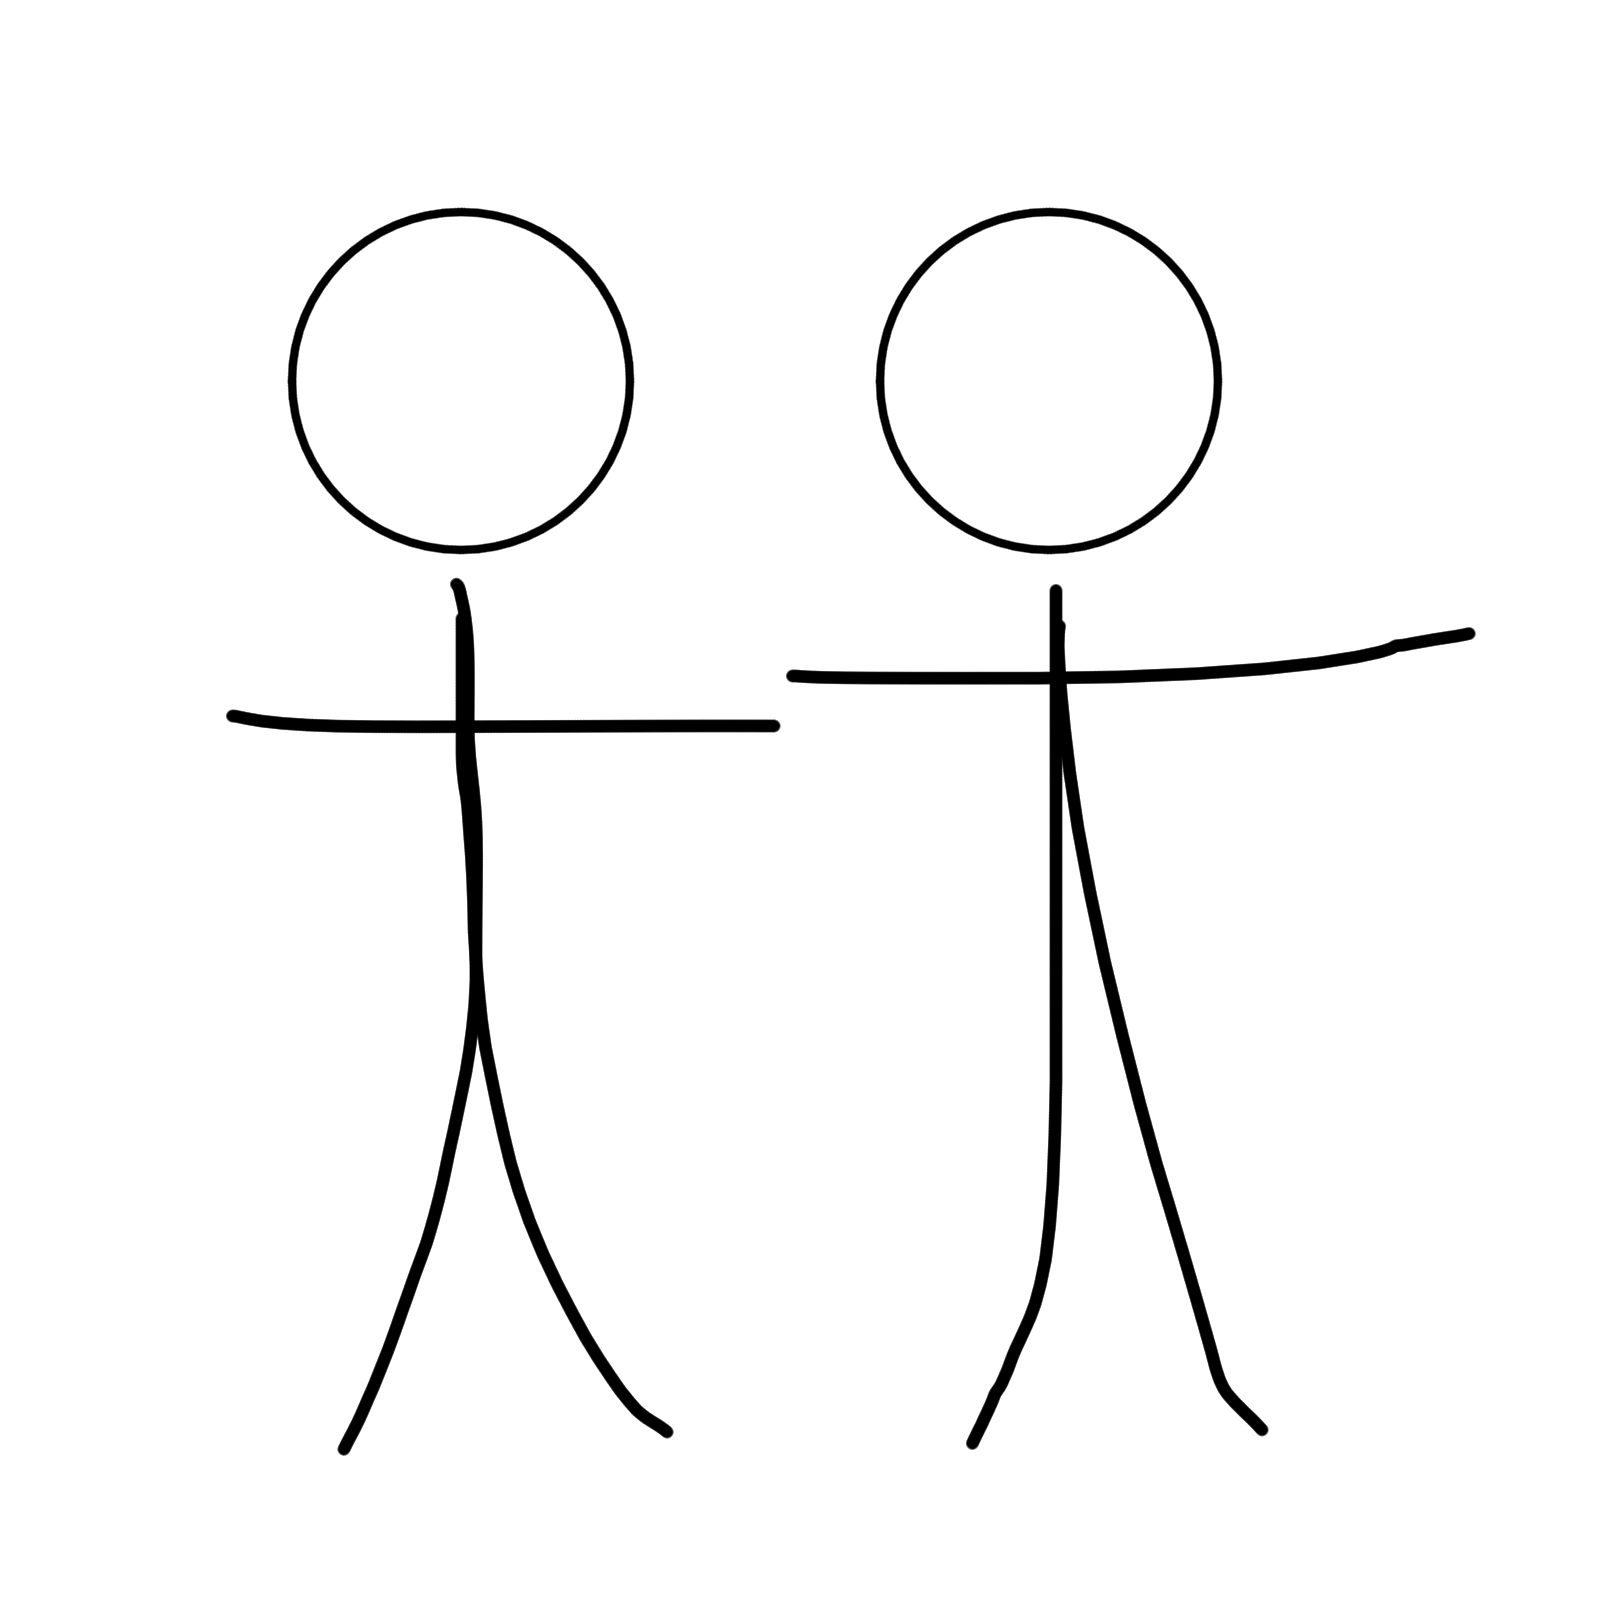
\includegraphics[width=\linewidth, height=20mm]{img/6loa_separate_keyframe}
    \end{minipage}
    & & & 
    \\ \hline
  \end{tabular}
  \caption{Types of Keyframes for Two Dancing Characters}
  \label{table:LOAChart}
\end{table}

There are 6 poses combinations for the characters separately. The asymmetrical poses for the odd number of LOAs can be mirrored (for 3 and 5 LOAs); therefore there are actually 8 poses for two characters separately. There are 10 combinations for the characters together, treated as one character. There are 2 poses which can be mirrored, so there are actually 12 poses together. Overall, 20 poses exist for 2 articulated humanoid characters.

\section{Space-time Sketching}


\section{Optimization Problems}
%\subsection{math/algorithms}
The Conjugate Residual Method for Constrained Minimization Problems -- 2015\\
Constrained Closed Loop Inverse Kinematics -- 2010

\section{Rig Combinations as Trees}
